\appendix

\chapter{Systematic Literature Review Supporting Materials}
\label{appendix:literature-review}

This appendix provides comprehensive supporting materials for the systematic literature review of collaborative augmented reality (AR) applications in industrial settings. The materials are organized into three main sections: the search methodology, screening process, and detailed coding sheets for the analysis of the 33 included papers.

\section{Search Strings}
\label{appendix:search-strings}

\subsection{Scopus Search String}

\begin{verbatim}
TITLE-ABS-KEY(("augmented reality" OR "mixed reality" OR "extended reality" OR 
"spatial computing" OR "head-mounted display" OR "smart glasses" OR "AR" OR 
"MR" OR "XR" OR "HMD")) AND TITLE-ABS-KEY((collaborat* OR cooperat* OR 
"shared experience" OR "multi-user" OR "peer-to-peer" OR teamwork OR 
"remote assistance" OR "shared workspace" OR "co-located" OR "synchronous" OR 
"asynchronous")) AND TITLE-ABS-KEY((industr* OR manufacturing OR factory OR 
production OR "assembly line" OR maintenance OR logistics OR "shop floor" OR 
"process industry" OR automotive OR aerospace OR shipbuilding)) AND NOT 
TITLE-ABS-KEY((gaming OR entertainment OR tourism OR medical OR healthcare OR 
retail OR marketing OR sports OR education OR "social media")) AND 
PUBYEAR > 2016 AND LANGUAGE(english)
\end{verbatim}

\subsection{IEEE Xplore Search String}

\begin{verbatim}
("All Metadata":("augmented reality" OR "mixed reality" OR "extended reality" OR 
"spatial computing" OR "head-mounted display" OR "smart glasses" OR "AR" OR 
"MR" OR "XR" OR "HMD")) AND ("All Metadata":(collaborat* OR cooperat* OR 
"shared experience" OR "multi-user" OR "peer-to-peer" OR teamwork OR 
"remote assistance" OR "shared workspace" OR "co-located" OR "synchronous" OR 
"asynchronous")) AND ("All Metadata":(industr* OR manufacturing OR factory OR 
production OR "assembly line" OR maintenance OR logistics OR "shop floor" OR 
"process industry" OR automotive OR aerospace OR shipbuilding)) NOT 
("All Metadata":(gaming OR entertainment OR tourism OR medical OR healthcare OR 
retail OR marketing OR sports OR education OR "social media"))
\end{verbatim}

Note: IEEE Xplore does not support publication year or language filters in the search interface; these were applied manually during export.

\subsection{ACM Digital Library Search String}

\begin{verbatim}
[All: "augmented reality" OR "mixed reality" OR "extended reality" OR 
"spatial computing" OR "head-mounted display" OR "smart glasses" OR "AR" OR 
"MR" OR "XR" OR "HMD"] AND [All: collaborat* OR cooperat* OR 
"shared experience" OR "multi-user" OR "peer-to-peer" OR teamwork OR 
"remote assistance" OR "shared workspace" OR "co-located" OR "synchronous" OR 
"asynchronous"] AND [All: industr* OR manufacturing OR factory OR production OR 
"assembly line" OR maintenance OR logistics OR "shop floor" OR 
"process industry" OR automotive OR aerospace OR shipbuilding] NOT 
[All: gaming OR entertainment OR tourism OR medical OR healthcare OR retail OR 
marketing OR sports OR education OR "social media"]
\end{verbatim}

Note: ACM Digital Library publication year filter (>2016) was applied using the interface controls. Language filtering was performed manually during screening.


\clearpage

\section{LLM-Assisted Screening Process}
\label{appendix:screening}
Full details can be found in the repository \url{https://github.com/gereonelvers/masters-thesis}.

\clearpage

\chapter{Literature Review Coding Sheets}
\label{appendix:coding-sheets}

This chapter presents the comprehensive coding sheets for the systematic literature review. The coding was conducted across three dimensions corresponding to the research questions, with each of the 33 included papers systematically analyzed and coded. The three coding sheets are:

\begin{itemize}
    \item \textbf{Types of Collaboration} (Section~\ref{appendix:types-collaboration}): Coding related to RQ1, examining application types, collaboration modes, and interaction mechanisms
    \item \textbf{Technical Implementation} (Section~\ref{appendix:technical-implementation}): Coding related to RQ2, examining hardware, software, and technical challenges
    \item \textbf{UX Design Approaches} (Section~\ref{appendix:ux-design}): Coding related to RQ3, examining user experience design patterns and effectiveness
\end{itemize}

\section{Types of Collaboration}
\label{appendix:types-collaboration}

Table~\ref{tab:coding-types-collaboration} presents the systematic coding of collaboration types and characteristics across all 33 papers. This coding sheet addresses RQ1 by examining the various forms of collaborative AR implementation, interaction mechanisms, and application contexts in industrial settings.

\afterpage{
\clearpage
\begin{landscape}
\tiny
\begin{longtable}{@{}p{1.8cm}p{1.8cm}p{1.8cm}p{1.8cm}p{1.8cm}p{1.8cm}p{1.8cm}p{1.8cm}@{}}
\caption{Coding sheet for Types of Collaboration (RQ1)} \label{tab:coding-types-collaboration} \\
\toprule
\textbf{Paper} & \textbf{Application Type} & \textbf{Collaboration Type} & \textbf{Interaction Mechanism} & \textbf{Application Context} & \textbf{Task Complexity} & \textbf{Evaluation Metrics} & \textbf{Use Case Effectiveness} \\
\midrule
\endfirsthead

\caption[]{Coding sheet for Types of Collaboration (RQ1) (continued)} \\
\toprule
\textbf{Paper} & \textbf{Application Type} & \textbf{Collaboration Type} & \textbf{Interaction Mechanism} & \textbf{Application Context} & \textbf{Task Complexity} & \textbf{Evaluation Metrics} & \textbf{Use Case Effectiveness} \\
\midrule
\endhead

\midrule
\multicolumn{8}{r}{\textit{Continued on next page}} \\
\endfoot

\bottomrule
\endlastfoot

Aschenbrenner et al. (2018) & Knowledge Transfer \& Expert Support & Co-located multi-user with remote expert & First-person video perspective, 3D object manipulation & Industrial production planning & High—step-by-step guidance & Task duration, error rate, usability ratings & Demonstrated improvements in efficiency and accuracy \\
\midrule
Aschenbrenner et al. (2019) & Knowledge Transfer \& Expert Support & Single-user and collaborative repair tasks & Visual annotations, audio/text instructions & Industrial robot maintenance & High—complex repair steps & Task duration, error rate, task load & Projection-based SAR significantly improved performance \\
\midrule
Betti et al. (2018) & Collaborative Creative Workflows & Multi-user, co-located design with non-professionals & Hand gestures and voice commands & Architectural design and fabrication & Moderate—CAD manipulation & Ease of use, user engagement, error rate & Holographic AR enabled productive interaction \\
\midrule
Buyruk and Çağdaş (2022) & Collaborative Creative Workflows & Multi-user collaboration in shared MR environment & Hand gestures and voice commands & Parametric design and fabrication & High—real-time design updates & Real-time responsiveness, user adaptability & High user engagement and efficiency \\
\midrule
Chan et al. (2022) & Precision Task Execution & Human-robot collaborative manufacturing & Gesture, speech, and gaze inputs & CFRP fabrication & High—trajectory adjustments & Task load, system usability & Enhanced engagement, reduced physical demand \\
\midrule
Cogurcu et al. (2023) & Precision Task Execution & Human-robot collaboration & Safety zones via HoloLens & Pick-and-place tasks & Moderate—safety zone management & Trust, safety perception & Increased safety and task ease \\
\midrule
De Franco et al. (2019) & Precision Task Execution & Human-robot collaboration & Gesture, gaze, and voice & Industrial assembly and polishing & Moderate—sequential coordination & Task performance, cognitive load & Improved coordination with real-time feedback \\
\midrule
Fang et al. (2022) & Precision Task Execution & Multi-operator, distributed assembly & Visual guidance overlays & Collaborative assembly on shop floors & High—multi-user synchronization & Localization accuracy, task efficiency & Improved task alignment and guidance \\
\midrule
Gemito et al. (2023) & Precision Task Execution & Human-robot collaboration & Visual/audio cues, step-by-step guidance & Automotive manufacturing & High—complex assembly & Task accuracy, safety perception & 30\% reduction in assembly time \\
\midrule
Goepel and Crolla (2020) & Collaborative Creative Workflows & Multi-user co-located creative assembly & Visual overlays, flow pattern guides & Bamboo art installation & High—sculptural alignment & User satisfaction, engagement & High flexibility and engagement \\
\midrule
Gursch et al. (2018) & Collaborative Creative Workflows & Human-robot collaboration in logistics & Real-time task updates, conflict alerts & Intralogistics and scheduling & High—conflict resolution & Task efficiency, user focus & Improved logistics coordination \\
\midrule
Huy et al. (2017) & Knowledge Transfer \& Expert Support & Co-located HRI with awareness modes & Laser-projected cues, see-through AR & Industrial task coordination & Moderate—real-time monitoring & Task engagement, safety perception & Enhanced awareness and safety \\
\midrule
Liu et al. (2018) & Dynamic Problem-Solving & Multi-user AR platform & 3D models, gaze indicators & Boat customization and sales & Moderate—interactive adjustments & Customer satisfaction, engagement & Enhanced customer experience \\
\midrule
Liu et al. (2022) & Knowledge Transfer \& Expert Support & Human-machine collaboration & Real-time instructions, quality monitoring & Aerospace assembly & High—precision alignment & Assembly efficiency, error rate & Improved accuracy and efficiency \\
\midrule
Lotsaris et al. (2021) & Knowledge Transfer \& Expert Support & Human-robot collaboration & Task instructions, robot control & Automotive assembly & Moderate—robot navigation & Task completion efficiency & Enhanced task accuracy \\
\midrule
Lu et al. (2021) & Precision Task Execution & Multi-user AR-based visualization & 3D sand table, environment visualization & Industrial park planning & Moderate—data visualization & System performance, user satisfaction & High user engagement \\
\midrule
Martins et al. (2024) & Knowledge Transfer \& Expert Support & Multi-user, multi-robot system & Real-time DT display, trajectory viewing & Industrial multi-robot environments & High—task coordination & Situational awareness, scalability & Improves safety and coordination \\
\midrule
Michalos et al. (2018) & Precision Task Execution & Industrial HRC system & Real-time AR instructions, smartwatch control & Automotive assembly & High—safety zone management & Cycle time reduction, safety incidents & Reduced physical load on operators \\
\midrule
Mourtzis et al. (2021) & Collaborative Creative Workflows & Multi-user collaborative design & 3D hologram manipulation, gestures & Manufacturing design & High—part customization & Design cycle time, user engagement & Reduced design cycle time \\
\midrule
Otto et al. (2016) & Knowledge Transfer \& Expert Support & Multi-user dual reality system & Real-time assembly visualization & Production planning & High—ergonomic evaluation & Error rate reduction, cycle time & Enhanced collaborative decision-making \\
\midrule
Putri et al. (2024) & Knowledge Transfer \& Expert Support & Collaborative safety system & Real-time visual cues, training simulations & Manufacturing safety & Moderate—hazard detection & Incident rate, response time & Improved safety communication \\
\midrule
Reis et al. (2021) & Precision Task Execution & Multi-user VR/AR simulation & Digital twin navigation, 3D manipulation & Offshore oil and gas & High—critical task simulations & Safety incident reduction & Reduced human exposure to risks \\
\midrule
Restas et al. (2024) & Precision Task Execution & Multi-user collaborative AR/VR & Real-time model customization & Social manufacturing & Moderate to high—customization & User engagement, communication effectiveness & Supports efficient co-creation \\
\midrule
Rogeau and Rezaei Rad (2024) & Knowledge Transfer \& Expert Support & Multi-level human-robot system & Holographic instructions, trajectory visualization & Timber assembly & High—complex joint fitting & Assembly accuracy, error reduction & Enhances precision and safety \\
\midrule
Rubart et al. (2022) & Precision Task Execution & Multimodal AR platform & Shared dashboards, gesture/voice control & Smart manufacturing control room & Moderate to high—monitoring & Situational awareness, response time & Enhanced real-time data access \\
\midrule
Schmidt et al. (2022) & Precision Task Execution & AR interface for HRI & Real-time robot metrics visualization & Robotic cell management & High—real-time monitoring & Cycle time, energy consumption & Enhances task efficiency and safety \\
\midrule
Stacchio et al. (2023) & Collaborative Creative Workflows & Collaborative MR platform & Holographic document interaction & Assembly task management & Moderate—document access & Task efficiency, error reduction & Enhances on-site productivity \\
\midrule
Verlinden and Bekker (2017) & Knowledge Transfer \& Expert Support & Multi-stakeholder AR platform & Holographic overlays with metrics & Urban infrastructure design & High—environmental analysis & Material efficiency, stakeholder alignment & Enhances environmental impact understanding \\
\midrule
Vidal-Balea et al. (2020) & Collaborative Creative Workflows & Industrial AR for training & Shared AR visualization & Shipbuilding training & Moderate—assembly guidance & Communication delay, transmission latency & Enhances task comprehension \\
\midrule
Wang et al. (2022) - Cross-platform & Precision Task Execution & Cross-platform AR communication & Real-time AR annotations & Shipbuilding assembly & Moderate to high—multi-device sync & Annotation accuracy, transmission latency & Enhances assembly coordination \\
\midrule
Wang et al. (2022) - Multi-person & Dynamic Problem-Solving & Multi-person collaborative AR & Role-based user interactions & Assembly process evaluation & High—role-specific tasks & Usability, task accuracy & Enhances assembly evaluation \\

Yang et al. (2023) & Collaborative Creative Workflows & Multi-user, non-dyadic AR & Task-specific holograms, role-based instruction & Timber prefabrication & High—coordinated task sharing & System Usability Scale, task accuracy & Facilitates coordinated task management \\
\end{longtable}
\end{landscape}
\clearpage
} 

\clearpage

\section{Technical Implementation}
\label{appendix:technical-implementation}

Table~\ref{tab:coding-technical-implementation} presents the systematic coding of technical implementation aspects across all 33 papers. This coding sheet addresses RQ2 by examining hardware platforms, software architectures, technical challenges, and resilience strategies employed in collaborative AR systems.

\afterpage{
\clearpage
\begin{landscape}
\tiny
\begin{longtable}{@{}p{1.8cm}p{1.8cm}p{1.8cm}p{1.8cm}p{1.8cm}p{1.8cm}p{1.8cm}p{1.8cm}@{}}
\caption{Coding sheet for Technical Implementation (RQ2)} \label{tab:coding-technical-implementation} \\
\toprule
\textbf{Paper} & \textbf{Hardware} & \textbf{Software and Tracking} & \textbf{Communication Latency} & \textbf{Field of View Limitations} & \textbf{Environmental Constraints} & \textbf{Error Sources} & \textbf{Resilience Strategies} \\
\midrule
\endfirsthead

\caption[]{Coding sheet for Technical Implementation (RQ2) (continued)} \\
\toprule
\textbf{Paper} & \textbf{Hardware} & \textbf{Software and Tracking} & \textbf{Communication Latency} & \textbf{Field of View Limitations} & \textbf{Environmental Constraints} & \textbf{Error Sources} & \textbf{Resilience Strategies} \\
\midrule
\endhead

\midrule
\multicolumn{8}{r}{\textit{Continued on next page}} \\
\endfoot

\bottomrule
\endlastfoot

Aschenbrenner et al. (2018) & Microsoft HoloLens, desktop interface & Custom HoloLens app, synchronized views & Low latency required for precision & Limited HoloLens FOV restricts workspace visibility & Lighting and space calibration critical & Object misalignment, real-time lag & Miniaturized views, enhanced spatial visualization \\
\midrule
Aschenbrenner et al. (2019) & Microsoft HoloLens, tablets, projection-based SAR & Metaio SDK, Android app & Low latency for visual alignment & Limited HoloLens FOV, projection-based superior coverage & Ambient lighting critical for projection & Collaborative task errors minimized with visual context & Projection-based AR minimized latency issues \\
\midrule
Betti et al. (2018) & Microsoft HoloLens, ABB 1200 robotic arm & Grasshopper and Python pipeline & Low latency critical for synchronization & Sensor inaccuracies in bright lighting & High lighting variability affected tracking & Sensor misinterpretation due to sun glare & Real-time feedback on interaction \\
\midrule
Buyruk and Çağdaş (2022) & HoloLens 2, Kuka KR210 robotic arm & Grasshopper3D, REST API with Unity & Low latency, near-instant updates & MR visuals enabled real-time overlay & Requires controlled lighting and calibration & Occasional robotic execution misalignments & Digital twin provided instant feedback \\
\midrule
Chan et al. (2022) & HoloLens, KUKA IIWA LBR14 & ROS Bridge, MoveIt library & Low latency for synchronized interaction & HoloLens drift affecting marker alignment & Speech recognition challenges in noise & AR tracking drift, marker misalignment & Positional recalibration via gaze \\
\midrule
Cogurcu et al. (2023) & Microsoft HoloLens 2, UR10 robot & Unity3D and ROS & Wi-Fi latency, additional safety layers & AR marker alignment drift & Network and tracking discrepancies & Safety zone misalignments due to drift & Recalibration prompts, digital twin synchronization \\
\midrule
De Franco et al. (2019) & Microsoft HoloLens, ROS-based Panda & Double-channel UDP, Unity3D, ROS & Low latency for synchronized updates & Voice commands affected by noise & Speech challenges in noisy environments & Voice misrecognition, hologram misalignment & Gesture-based commands as backup \\
\midrule
Fang et al. (2022) & Microsoft HoloLens 2, ROS-based mobile robot & Visual-inertial SLAM, ROS localization & Managed through visual-inertial SLAM & High accuracy 3D model alignment required & Large industrial spaces, dynamic conditions & Drift in visual tracking & Incremental triangulation reduces drift \\
\midrule
Gemito et al. (2023) & Microsoft HoloLens 2, FIWARE and ROS2 & Unity MRTK, Holographic Remoting & Holographic Remoting provided real-time visualization & Requires precise calibration & Variable lighting can impact visibility & Calibration issues, real-time misalignment & Holographic safety barrier reduces risk \\
\midrule
Goepel and Crolla (2020) & Microsoft HoloLens, smartphones & Anemone plugin in Rhino & Managed through unified overlays & Flexible calibration for material irregularities & Natural variability of bamboo & Material variations, AR markers misaligned & Adaptable guidance, procedural modeling \\
\midrule
Gursch et al. (2018) & AR and VR devices & EIS for real-time updates & Real-time data processing & Not explicitly addressed & Efficient scheduling adaptation & Potential for information overload & Adaptive filtering based on eye-tracking \\
\midrule
Huy et al. (2017) & Epson Moverio BT-200, MAVEN robot & Marker-based tracking, laser-projected SAR & Real-time synchronization & Laser-writer improves outdoor visibility & Laser visibility in bright environments & AR marker misalignment & Gestures and haptic inputs allow adjustments \\
\midrule
Liu et al. (2018) & Microsoft HoloLens, Vuforia markers & Unity3D, Vuforia markers & Real-time synchronization maintained & Marker-based tracking, lighting influences & Flexible with markers, lighting impacts & Tracking inaccuracies in varying lighting & Conflict management, marker relocation \\
\midrule
Liu et al. (2022) & Wearable AR devices, Digital Twin & Digital Twins, Knowledge Graph & Real-time synchronization & Marker-based tracking enables alignment & Optimized for variable lighting & Assembly misalignments & Dynamic tolerance allocation \\
\midrule
Lotsaris et al. (2021) & Microsoft HoloLens, ROS-based platform & Digital Twin, QR code calibration & Real-time updates for robot interaction & Flexible to lighting variations & Complex task environments & Tracking issues with QR codes & Direct robot control, safety monitoring \\
\midrule
Lu et al. (2021) & Microsoft HoloLens, desktop PC & VRML for 3D models, YOLOv2 & Real-time data synchronization & VRML-based, performance-optimized & Adaptable to lighting conditions & Interaction conflicts in multi-user & VRML model optimizations \\
\midrule
Martins et al. (2024) & Microsoft HoloLens 2, ROS Noetic & ROS navigation, Map Frame Matcher & Wi-Fi communication, low latency & QR code-based alignment & Scalability limits with port-based communication & Possible alignment drift & Real-time updates, safety zones \\
\midrule
Michalos et al. (2018) & Epson Moverio, Motorola Moto 360 & ROS-based architecture, SafetyEye 3D & Real-time Wi-Fi updates & SafetyEye dynamic zones & Adaptable warning/danger zones & Potential AR-based guidance missteps & SafetyEye dynamic zones, emergency stop \\
\midrule
Mourtzis et al. (2021) & Microsoft HoloLens, cloud-based MR & Voxel-based modeling, CNN & Real-time cloud synchronization & Stable MR rendering & Efficient voxel modeling for AM & Misalignment mitigated by algorithms & Cloud-based recovery, voxel modeling \\
\midrule
Otto et al. (2016) & Powerwalls, Microsoft PixelSense & VRPN and ARVIDA protocols & Real-time visualization & Large-scale, true-to-scale displays & Optimized for industrial environments & Misalignment in spatial projection & Layered physical-virtual feedback \\
\midrule
Putri et al. (2024) & AR headsets, wearable sensors & IoT-enabled wearables & Immediate alerts for hazard prevention & User-centered AR, minimal distraction & High-noise, high-hazard manufacturing & Potential alert saturation & Wearable alerts, real-time visual cues \\
\midrule
Reis et al. (2021) & HTC Vive, Microsoft HoloLens & Unity engine, VRPN & Real-time data access from digital twin & AR limited by model size & High-risk FPSO settings & Potential for spatial lag & Safety zones, error correction \\
\midrule
Restas et al. (2024) & Web VR, Mobile AR, HoloLens & Unity-based with API integration & Real-time cross-device synchronization & Web VR and HoloLens adapted & Flexible across platforms & Potential sync lag & API integration, real-time updates \\
\midrule
Rogeau and Rezaei Rad (2024) & Microsoft HoloLens 2, ABB 6400 & Grasshopper, Rhinoceros, Python & Real-time updates for task guidance & Holographic projection for adjustments & Variable workspace conditions & Potential alignment drift & Task allocation, AR support \\
\midrule
Rubart et al. (2022) & Microsoft HoloLens 2, tablets & Unity, MRTK, OPC UA protocol & Real-time data and alert syncing & AR provides mobile data access & Static and mobile control rooms & Tracking errors in dynamic environments & Multimodal inputs, shared annotations \\
\midrule
Schmidt et al. (2022) & Microsoft HoloLens 2 & Unity, MRTK, MQTT & Real-time synchronization via MQTT & HoloLens for real-time feedback & Dynamic robotic cell environments & Tracking errors in dynamic setup & Task-specific visual alerts \\
\midrule
Stacchio et al. (2023) & Microsoft HoloLens 2 & Unity, MRTK, REST API & Minimal, asynchronous updates & MR interface optimized for documents & Assembly environments & Annotation management errors & Asynchronous annotation sharing \\
\midrule
Verlinden and Bekker (2017) & Microsoft HoloLens & 3D scanning, WAAM scorecards & Real-time data and design sync & Large-scale outdoor visualization & Outdoor-ready with 3D scans & Model misalignment in dynamic conditions & Material efficiency data, real-time feedback \\
\midrule
Vidal-Balea et al. (2020) & Microsoft HoloLens & Unity, custom UDP-TCP protocol & Low latency, delays below 5 ms & Large-scale assembly adaptation & Shipyard-ready, 5 GHz WiFi & Potential sync delays & Anchor synchronization, packet redundancy \\
\midrule
Wang et al. (2022) - Cross-platform & Microsoft HoloLens 2 & Unity, custom UDP-TCP & Low latency, asynchronous updates & Large shipyard spaces & Metal-dense, large-scale shipyards & Desync or misalignment & Multi-device sync, cloud redundancy \\
\midrule
Wang et al. (2022) - Multi-person & Microsoft HoloLens 2, Azure Kinect & Unity, marker-based alignment & Low latency, real-time sync & Spatial manipulation optimization & Precision-focused, stable alignment & Desync in role-based tasks & Synchronized multi-user environment \\

Yang et al. (2023) & Microsoft HoloLens 2, Surface Pro & Unity, VIZOR, ROS backend & Low latency, real-time synchronization & Large timber structures & Prefabrication sites & Task misalignment & Task prompts, role-specific coordination \\
\end{longtable}
\end{landscape}
\clearpage
} 

\clearpage

\section{UX Design Approaches}
\label{appendix:ux-design}

Table~\ref{tab:coding-ux-design} presents the systematic coding of user experience design approaches across all 33 papers. This coding sheet addresses RQ3 by examining design patterns, user satisfaction metrics, and evidence of effectiveness in collaborative AR systems.

\afterpage{
\clearpage
\begin{landscape}
\tiny
\begin{longtable}{@{}p{1.8cm}p{1.8cm}p{1.8cm}p{1.8cm}p{1.8cm}p{1.8cm}p{1.8cm}p{1.8cm}@{}}
\caption{Coding sheet for UX Design Approaches (RQ3)} \label{tab:coding-ux-design} \\
\toprule
\textbf{Paper} & \textbf{Design Approach} & \textbf{User Experience Focus} & \textbf{Evidence of Effectiveness} & \textbf{Collaborative Interaction Design} & \textbf{User Satisfaction Metrics} & \textbf{Adaptability} & \textbf{Grounding Effects} \\
\midrule
\endfirsthead

\caption[]{Coding sheet for UX Design Approaches (RQ3) (continued)} \\
\toprule
\textbf{Paper} & \textbf{Design Approach} & \textbf{User Experience Focus} & \textbf{Evidence of Effectiveness} & \textbf{Collaborative Interaction Design} & \textbf{User Satisfaction Metrics} & \textbf{Adaptability} & \textbf{Grounding Effects} \\
\midrule
\endhead

\midrule
\multicolumn{8}{r}{\textit{Continued on next page}} \\
\endfoot

\bottomrule
\endlastfoot
Aschenbrenner et al. (2018) & Shared 3D spatial views, "Godmode" miniaturized view & Enhancing spatial awareness, reducing errors & Demonstrated reductions in task time and accuracy & Real-size AR for local users, miniaturized for remote experts & Ease of use, task satisfaction, situational awareness & Flexible, customizable views & Synchronized annotations improve understanding \\
\midrule
Aschenbrenner et al. (2019) & Shared 3D spatial views, projection and annotation & Enhancing user confidence, reducing cognitive load & SAR significantly reduced task duration and errors & Remote and local users with synchronized annotations & Projection-based SAR rated highest for usability & Flexible SAR setup & Strong grounding effects with SAR \\
\midrule
Betti et al. (2018) & Multimodal AR interface with task-specific icons & Accessible interface, minimal training & Positive usability feedback & Sequential collaboration model & High adaptability, positive reception & Flexible inputs, limited by time & Participants oriented well with AR cues \\
\midrule
Buyruk and Çağdaş (2022) & Digital twin in mixed reality & Real-time feedback for design-to-production & Enhanced user satisfaction & Shared MR environment for synchronized updates & Positive for usability and responsiveness & Highly adaptable to user inputs & MR-based instant feedback improved engagement \\
\midrule
Chan et al. (2022) & HMD interface to reduce cognitive load & Reduce physical strain, increase engagement & Higher usability scores over joystick & Shared interface for robot interaction & Highly rated for stimulation and novelty & Real-time robot adjustments & Improved task engagement through co-location \\
\midrule
Cogurcu et al. (2023) & Safety zones in MR with cage bars & Increasing user confidence in safety & High satisfaction with cage-bar design & Safety visualization improved coordination & Preferred cage-bar zones for real robots & Safety zone configurations adjustable & Improved spatial awareness with cage bars \\
\midrule
De Franco et al. (2019) & Non-intrusive feedback system & Streamlined task flow, minimal intrusiveness & Improved satisfaction, reduced mental load & User-controlled task scheduling & High preference for AR over screen-based & Adaptive to noise via gestures & Enhanced task focus with immersive AR \\
\midrule
Fang et al. (2022) & Adaptive, immersive visual guidance & Enhances situational awareness & Improved synchronization for large assemblies & Dynamic guidance based on individual locations & Ease of coordination reported & Highly adaptable for multi-user environments & Shared spatial context improves awareness \\
\midrule
Gemito et al. (2023) & Step-by-step visual instructions & Clarity, safety, reduced learning curve & 30\% assembly time reduction, 50\% learning time reduction & Facilitates task handoffs between human-robot & High satisfaction with adaptive workspace & Customizable workspace & Step tracking improved task flow \\
\midrule
Goepel and Crolla (2020) & Iterative, procedural guidance & Supported creative freedom with structural integrity & High user satisfaction & Synchronized model for collective alignment & Positive for intuitiveness and freedom & Allowed deviations due to material properties & Improved spatial understanding \\
\midrule
Gursch et al. (2018) & Context-specific AR guidance & Minimized cognitive load & Enhanced situational awareness & Humans monitor while robots handle routine & Positive feedback for adaptability & High, prioritizes info based on attention & Focused information delivery \\
\midrule
Huy et al. (2017) & Laser-projected SAR for public awareness & Improved situational awareness & Enhanced task flow and safety perception & Separate interfaces prevent overload & Positive feedback for adaptability & Laser cues adjustable to lighting & Dual-channel approach improves awareness \\
\midrule
Liu et al. (2018) & Interactive 3D renderings and animations & Increased customer satisfaction & Positive dealer feedback & Shared AR space with synchronized views & Positive reception for accessibility & Marker system provided flexibility & Enhanced awareness with avatars \\
\midrule
Liu et al. (2022) & Human-centric, adaptive task guidance & Reduces cognitive load & Enhanced task satisfaction & Synchronized task management through DTs & Positive feedback on cognitive load reduction & Real-time adaptation to operator state & Enhanced task clarity \\
\midrule
Lotsaris et al. (2021) & User-friendly, gesture-based interface & Enhances confidence with real-time updates & Increased task accuracy & Dynamic task reassignment & Positive for task engagement & Flexible for complex task flows & Safety visualization improves awareness \\
\midrule
Lu et al. (2021) & Immersive browsing with environmental data & Enhances collaborative planning & High user engagement & Consistent spatial orientation & Positive for immersive environment & Optimized VRML models & Interactive 3D models improve understanding \\
\midrule
Martins et al. (2024) & App bar controls for flexible task engagement & Enhances situational awareness & Positive feedback for safe control & Shared DT updates across users & High satisfaction for safety & Scalable but limited by port constraints & Improves alignment with robot paths \\
\midrule
Michalos et al. (2018) & Safety-first design with real-time AR & Minimizes cognitive load and physical strain & Improved task precision and safety & Adaptive AR interfaces & Positive feedback on task clarity & Highly adaptive to operator needs & Clear AR prompts reduce errors \\
\midrule
Mourtzis et al. (2021) & Gesture-based control, real-time feedback & Reduces cognitive load & Improved design speed and accuracy & Shared views and synchronized updates & High user satisfaction for flexibility & Flexible for large models & Clear visualization enhances engagement \\
\midrule
Otto et al. (2016) & Dual-reality with SAR, powerwall & Real-time interaction for error detection & Improved team collaboration & Shared displays support communication & Positive for adaptability & Highly adaptable to assembly tasks & Layered spatial cues enhance engagement \\
\midrule
Putri et al. (2024) & User-centered design with real-time alerts & Reduces cognitive load & Increased employee empowerment & Consolidated safety data platform & Positive feedback on usability & High adaptability for dynamic tasks & Enhanced safety culture through feedback \\
\midrule
Reis et al. (2021) & Safety-focused with intuitive VR/AR controls & Enhanced safety through immersive training & Positive feedback on usability & Supports collaborative tasks in VR & High user satisfaction for safety & Flexible for various training scenarios & Clear visual cues for high-risk tasks \\
\midrule
Restas et al. (2024) & Intuitive multi-device interface & Enhances co-creation & Effective for product customization & Synchronized across platforms & High satisfaction for adaptability & Highly adaptable for social manufacturing & Consistent views foster shared understanding \\
\midrule
Rogeau and Rezaei Rad (2024) & Holographic AR interface & Reduces cognitive load & Improved precision and control & Shared AR holograms align interaction & High satisfaction for task adaptability & Flexible in human-robot mixed assembly & Holograms reinforce task understanding \\
\midrule
Rubart et al. (2022) & User-friendly AR with gesture/voice control & Reduces cognitive load & Enhanced comprehension of complex data & Shared holograms, collaborative dashboards & Positive feedback for multimodal interaction & Adaptable for different control rooms & Visual cues support shared understanding \\
\midrule
Schmidt et al. (2022) & User-centered AR with task-specific overlays & Reduces cognitive load & Improved safety and decision accuracy & Shared real-time holographic views & Positive feedback on usability & Flexible for diverse robotic tasks & Clear visual cues improve awareness \\
\midrule
Stacchio et al. (2023) & Hands-free, customizable MR document interface & Reduces cognitive load & Improved task efficiency & Asynchronous annotations enable shared understanding & High adaptability & Flexible for diverse assembly tasks & Holographic documents support alignment \\
\midrule
Verlinden and Bekker (2017) & In-situ, data-driven AR interface & Real-time feedback reduces cognitive load & Improved decision-making & Shared holographic views & High adaptability to infrastructure projects & Flexible for various urban projects & Holographic projections reinforce understanding \\
\midrule
Vidal-Balea et al. (2020) & Simple interface with floating control panel & Streamlines training & Reduces reliance on paper manuals & Synchronized AR content & Positive for usability & Adaptable for shipbuilding & AR overlays provide real-time awareness \\
\midrule
Wang et al. (2022) - Cross-platform & Cross-device AR interface & Clear, layered feedback & Improves task alignment & Synchronized multi-device interface & Positive feedback & Adaptable to shipbuilding & Annotations aid quick location finding \\
\midrule
Wang et al. (2022) - Multi-person & Role-based AR interface & Real-time visual cues & Good usability (SUS score 71) & Shared AR space with role-specific tasks & Positive feedback & Adaptable to complex assembly & Visual aids enhance awareness \\

Yang et al. (2023) & Role-based AR UI with task-specific panels & Clear, context-driven instructions & 73.5 SUS score & Real-time task sync across users & Positive for situational awareness & Flexible for task-based role switching & 3D task representations facilitate flow \\
\end{longtable}
\end{landscape}
\clearpage
} 

\clearpage

\chapter{User Study Materials}
\label{appendix:anchors}

This appendix contains the materials used in the user study, including the Vuforia image targets for spatial anchoring and the participant documentation.

\section{Vuforia Image Targets}

The following pages show the sample image targets provided by Vuforia, retrieved from \url{https://developer.vuforia.com/library/vuforia-engine/images-and-objects/sample-apps-target-pdfs/}. These targets were used as anchors in the prototype implementation to establish spatial positioning and tracking in the augmented reality environment.

\includepdf[pages=1-3]{assets/appendix/vuforia_image_targets.pdf}

\section{User Study Documentation}

The following documents were provided to participants during the user study recruitment and consent process.

\subsection{User Study Information Sheet}

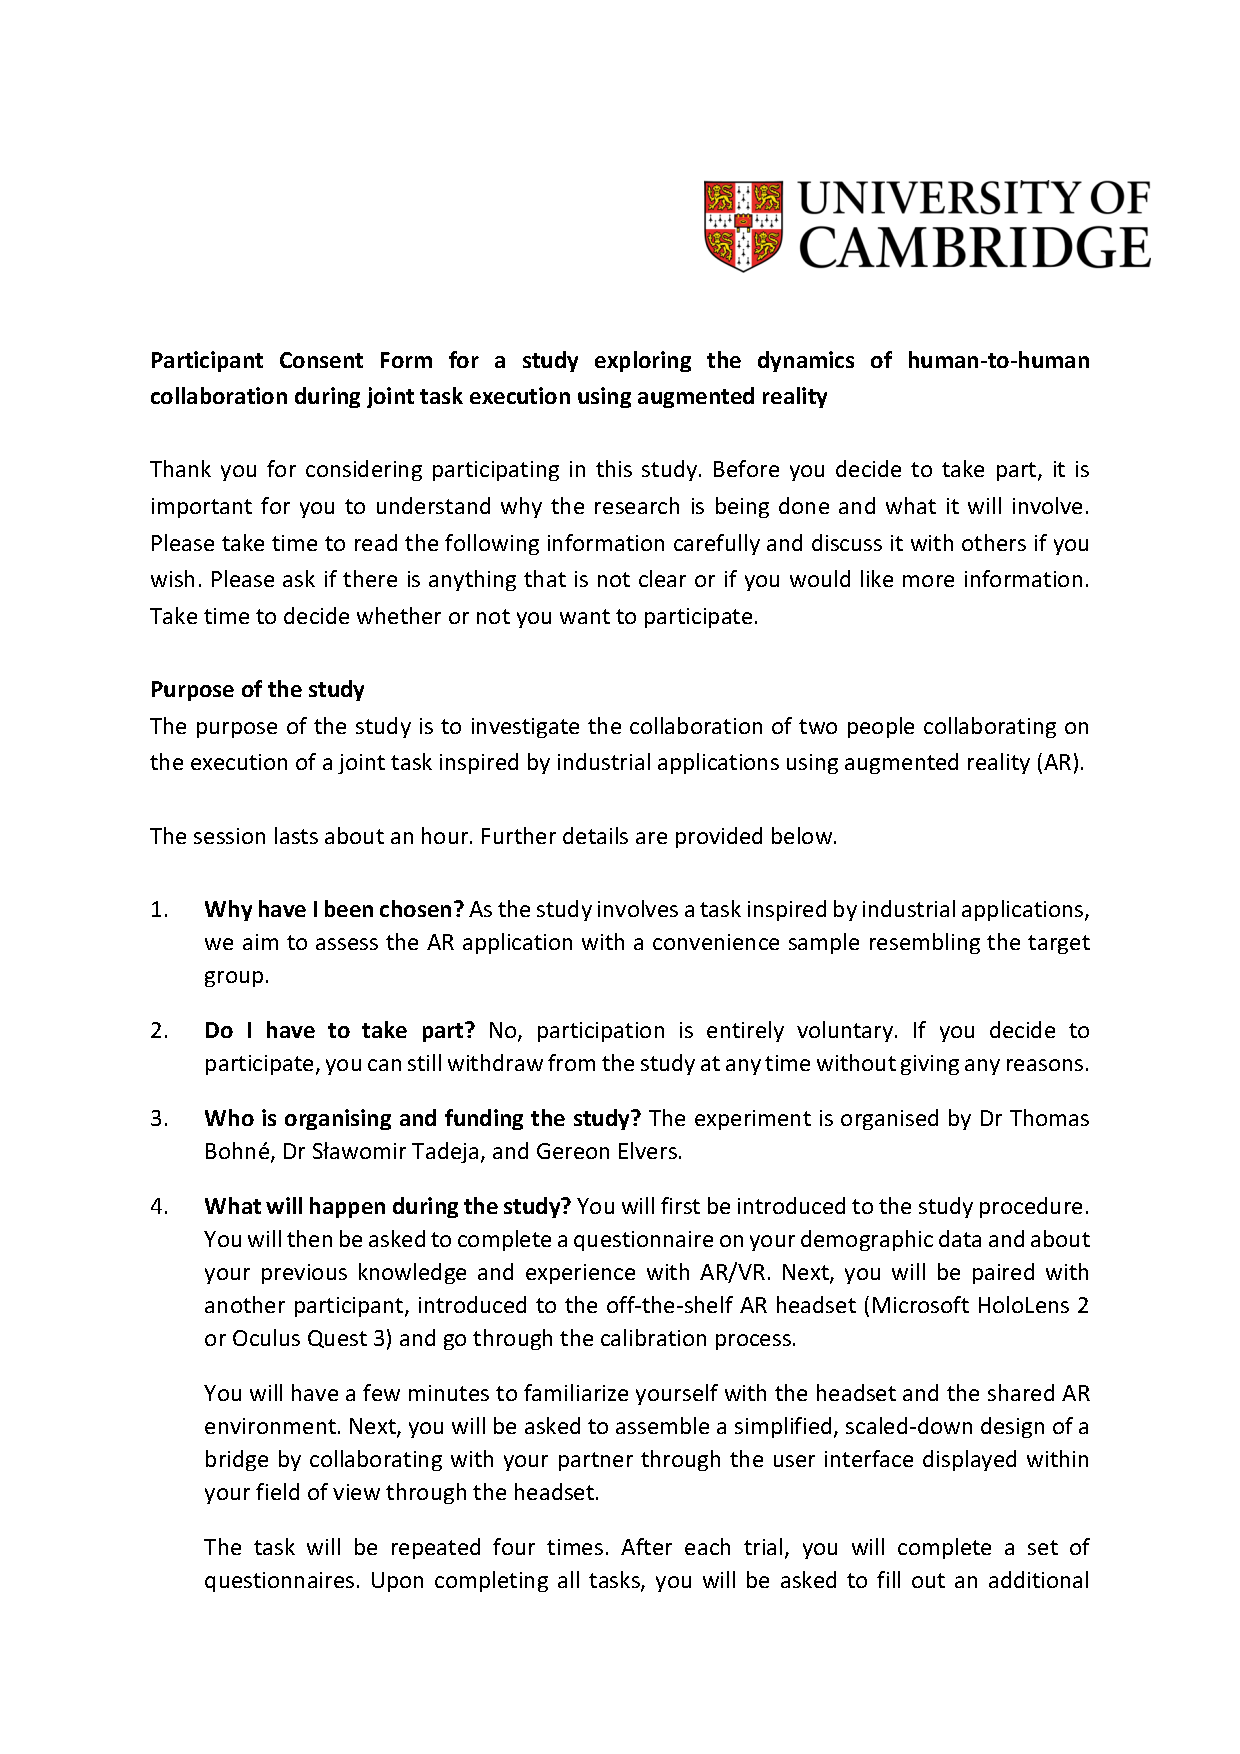
\includepdf[pages=-]{assets/appendix/user-study-info-sheet.pdf}

\subsection{User Study Consent Form}

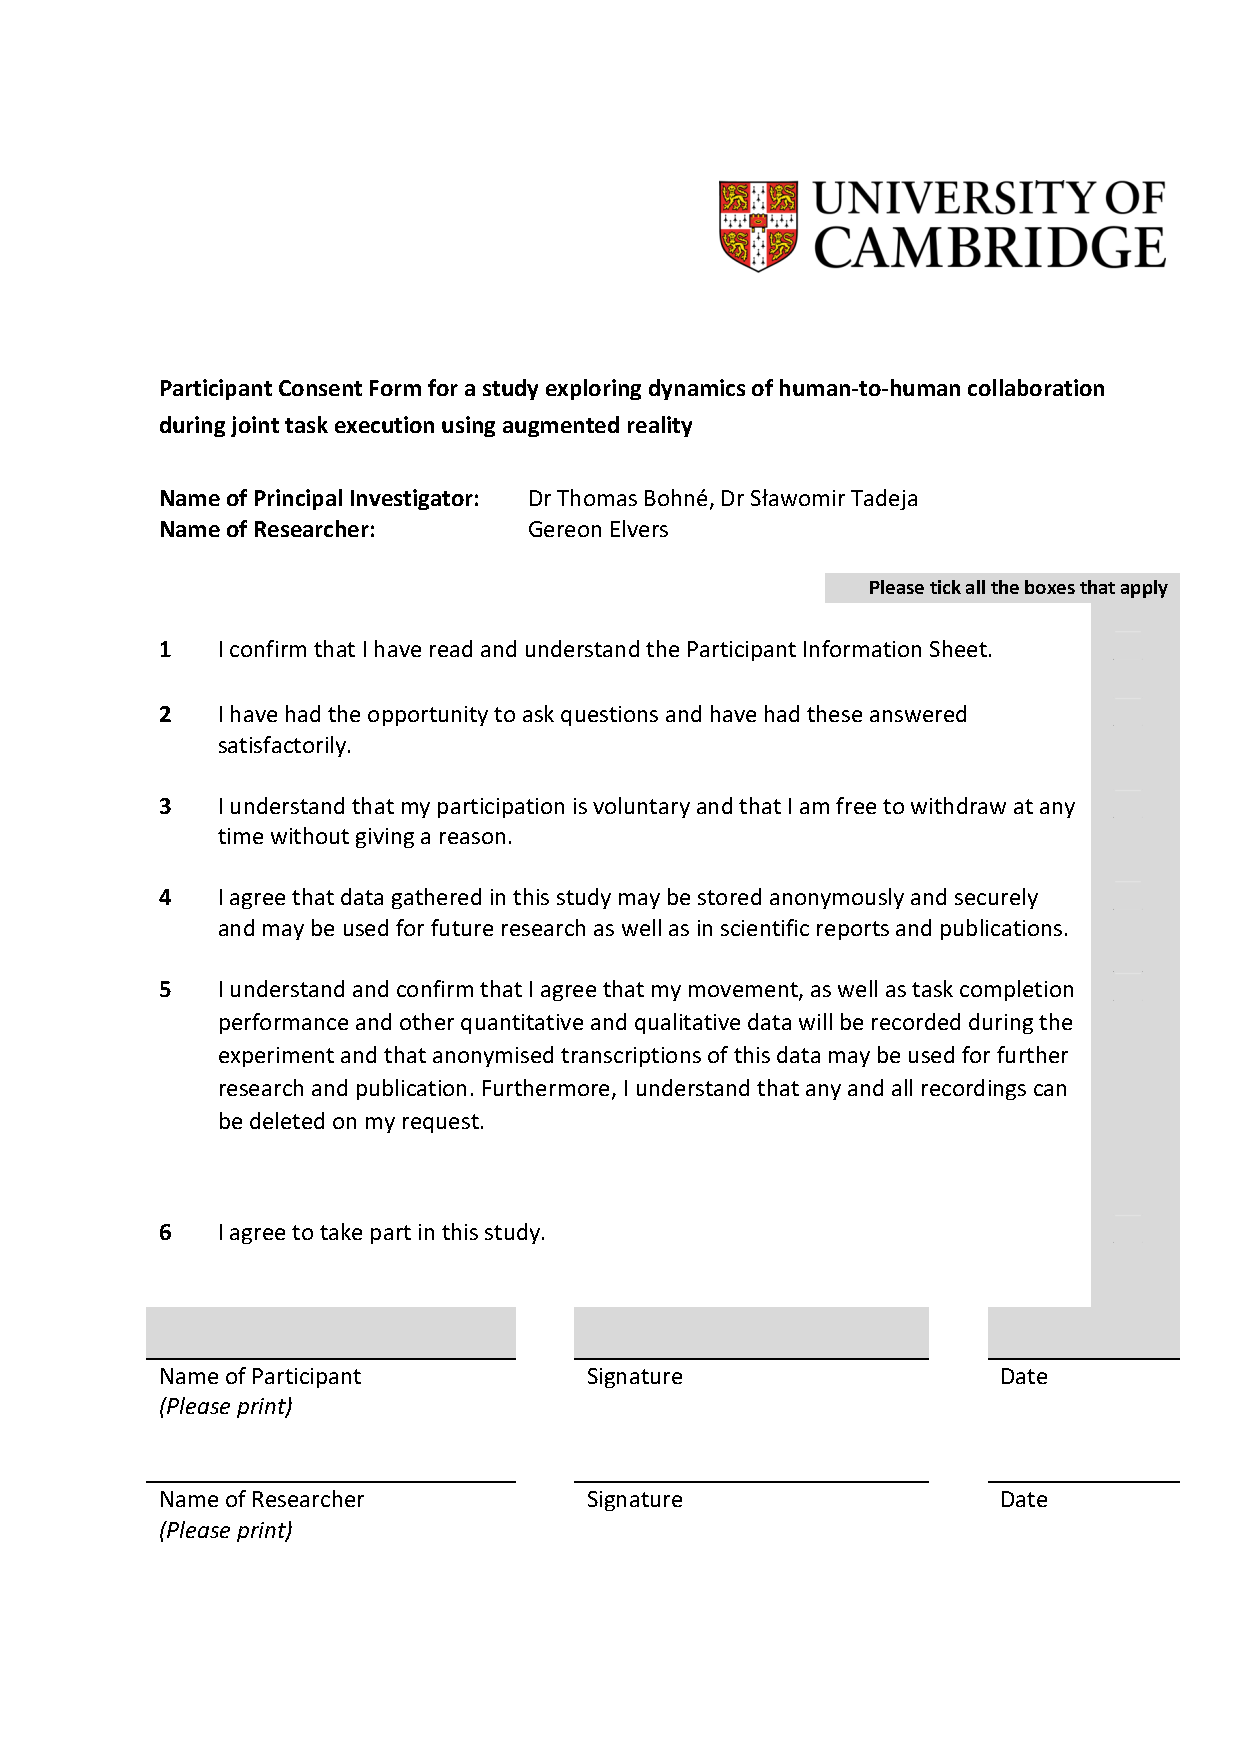
\includepdf[pages=-]{assets/appendix/user-study-consent-form.pdf}

\subsection{Introductory Presentation}

Each pair of participants received an introductory presentation before the start of the user study to familiarize them with the augmented reality system and the collaborative task. The presentation materials can be found in the thesis repository at \url{https://github.com/gereonelvers/masters-thesis}. 

\clearpage

\chapter{User Study Questionnaires and Interview Protocols}
\label{appendix:questionnaires}

This appendix contains the complete questionnaires and interview protocols used in the user study. The materials are organized into two main sections: standardized questionnaires and interview protocols.

\section{Standardized Questionnaires}

\subsection{Demographic Questionnaire}
\label{appendix:demographic-questionnaire}

The demographic questionnaire collected background information about participants and their relevant experience.

\begin{enumerate}
    \item Please select your gender:
    \begin{itemize}
        \item Male
        \item Female
        \item Non-binary
        \item Prefer not to say
        \item Enter yourself
    \end{itemize}
    
    \item Please state your age: \underline{\hspace{3cm}}
    
    \item What is your native language? \underline{\hspace{5cm}}
    
    \item Please select your current employment status:
    \begin{itemize}
        \item Student (incl. PhD)
        \item Staff
        \item Enter yourself
    \end{itemize}
    
    \item How would you rate your experience with Augmented Reality (AR) and Virtual Reality (VR) applications?
    \begin{itemize}
        \item No experience
        \item Limited experience
        \item Moderate experience
        \item Extensive experience
    \end{itemize}
    
    \item If applicable, please specify the AR/VR devices or applications you have used: \underline{\hspace{8cm}}
    
    \item What types of AR/VR applications have you interacted with? (Select all that apply)
    \begin{itemize}
        \item Gaming
        \item Training/Simulation
        \item Industrial Prototyping
        \item Collaboration
        \item Other
    \end{itemize}
    
    \item How would you rate your experience with assembly or prototyping tasks (e.g., building models, using CAD, working with physical kits)?
    \begin{itemize}
        \item No experience
        \item Limited experience
        \item Moderate experience
        \item Extensive experience
    \end{itemize}
    
    \item What tools or methods have you used for assembly or prototyping? \underline{\hspace{8cm}}
    
    \item If applicable, please describe any relevant experience with assembly or prototyping tasks: \underline{\hspace{8cm}}
    
    \item Do you have any additional concerns or comments? \underline{\hspace{8cm}}
\end{enumerate}

\subsection{Big Five Personality Inventory (BFI-50)}
\label{appendix:big-five}

Participants rated each statement on a 5-point Likert scale: \textbf{Strongly Disagree} - \textbf{Disagree} - \textbf{Neutral} - \textbf{Agree} - \textbf{Strongly Agree}

\begin{enumerate}
    \item Am the life of the party.
    \item Feel little concern for others.
    \item Am always prepared.
    \item Get stressed out easily.
    \item Have a rich vocabulary.
    \item Don't talk a lot.
    \item Am interested in people.
    \item Leave my belongings around.
    \item Am relaxed most of the time.
    \item Have difficulty understanding abstract ideas.
    \item Feel comfortable around people.
    \item Insult people.
    \item Pay attention to details.
    \item Worry about things.
    \item Have a vivid imagination.
    \item Keep in the background.
    \item Sympathize with others' feelings.
    \item Make a mess of things.
    \item Seldom feel blue.
    \item Am not interested in abstract ideas.
    \item Start conversations.
    \item Am not interested in other people's problems.
    \item Get chores done right away.
    \item Am easily disturbed.
    \item Have excellent ideas.
    \item Have little to say.
    \item Have a soft heart.
    \item Often forget to put things back in their proper place.
    \item Get upset easily.
    \item Do not have a good imagination.
    \item Talk to a lot of different people at parties.
    \item Am not really interested in others.
    \item Like order.
    \item Change my mood a lot.
    \item Am quick to understand things.
    \item Don't like to draw attention to myself.
    \item Take time out for others.
    \item Shirk my duties.
    \item Have frequent mood swings.
    \item Use difficult words.
    \item Don't mind being the center of attention.
    \item Feel others' emotions.
    \item Follow a schedule.
    \item Get irritated easily.
    \item Spend time reflecting on things.
    \item Am quiet around strangers.
    \item Make people feel at ease.
    \item Am exacting in my work.
    \item Often feel blue.
    \item Am full of ideas.
\end{enumerate}

\subsection{NASA Task Load Index (NASA-TLX)}
\label{appendix:nasa-tlx}

Participants rated each dimension on a scale from 0 to 100 in steps of 5, completed after each task variant.

\begin{enumerate}
    \item \textbf{Mental Demand:} How much mental and perceptual activity was required? Was the method easy or demanding, simple or complex?
    \begin{center}
        \begin{tabular}{|c|c|c|c|c|}
        \hline
        0 & 25 & 50 & 75 & 100 \\
        \hline
        Low & & & & High \\
        \hline
        \end{tabular}
    \end{center}
    
    \item \textbf{Physical Demand:} How much physical activity was required? Was the method easy or demanding, slack or strenuous?
    \begin{center}
        \begin{tabular}{|c|c|c|c|c|}
        \hline
        0 & 25 & 50 & 75 & 100 \\
        \hline
        Low & & & & High \\
        \hline
        \end{tabular}
    \end{center}
    
    \item \textbf{Temporal Demand:} How much time pressure did you feel due to the pace at which the method or method elements occurred? Was the pace slow or rapid?
    \begin{center}
        \begin{tabular}{|c|c|c|c|c|}
        \hline
        0 & 25 & 50 & 75 & 100 \\
        \hline
        Low & & & & High \\
        \hline
        \end{tabular}
    \end{center}
    
    \item \textbf{Performance:} How successful were you in performing the method? How satisfied were you with your performance?
    \begin{center}
        \begin{tabular}{|c|c|c|c|c|}
        \hline
        0 & 25 & 50 & 75 & 100 \\
        \hline
        Poor & & & & Perfect \\
        \hline
        \end{tabular}
    \end{center}
    
    \item \textbf{Effort:} How hard did you have to work (mentally and physically) to accomplish your level of performance?
    \begin{center}
        \begin{tabular}{|c|c|c|c|c|}
        \hline
        0 & 25 & 50 & 75 & 100 \\
        \hline
        Low & & & & High \\
        \hline
        \end{tabular}
    \end{center}
    
    \item \textbf{Frustration:} How irritated, stressed, and annoyed versus content, relaxed, and complacent did you feel during the method steps?
    \begin{center}
        \begin{tabular}{|c|c|c|c|c|}
        \hline
        0 & 25 & 50 & 75 & 100 \\
        \hline
        Low & & & & High \\
        \hline
        \end{tabular}
    \end{center}
\end{enumerate}

\subsection{System Usability Scale (SUS)}
\label{appendix:sus}

Participants rated each statement on a 5-point Likert scale: \textbf{Strongly Disagree} - \textbf{Disagree} - \textbf{Neutral} - \textbf{Agree} - \textbf{Strongly Agree}. This questionnaire was completed after each task variant.

\begin{enumerate}
    \item I think that I would like to use this system frequently.
    \item I found the system unnecessarily complex.
    \item I thought the system was easy to use.
    \item I think that I would need the support of a technical person to use this system.
    \item I found the various functions in this system were well integrated.
    \item I thought there was too much inconsistency in this system.
    \item I would imagine that most people would learn to use this system very quickly.
    \item I found the system very cumbersome to use.
    \item I felt very confident using the system.
    \item I needed to learn a lot of things before I could get going with this system.
\end{enumerate}

\subsection{Inclusion of Other in the Self (IOS) Scale}
\label{appendix:ios}

Participants selected one of seven pictorial options showing varying degrees of overlap between two circles representing themselves and their partner. This scale was administered twice: once before the study and once after.

\textbf{Question:} Which picture best describes your relationship with the other participant?

\begin{figure}[h]
\centering
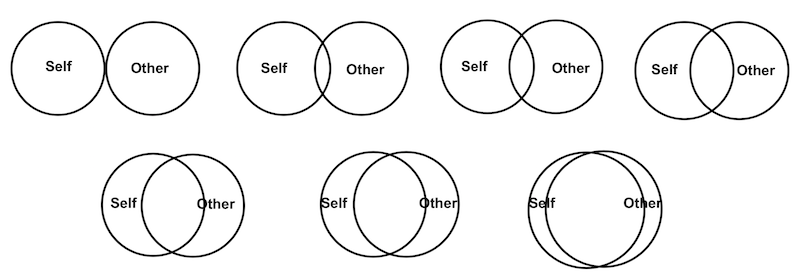
\includegraphics[width=0.8\textwidth]{assets/appendix/ios-circles.png}
\caption{The Inclusion of Other in the Self (IOS) Scale showing seven options with increasing degrees of overlap between "Self" and "Other" circles. Adapted from \cite{aron1991close}.}
\label{fig:ios-scale}
\end{figure}

Participants selected from Option 1 (no overlap) to Option 7 (almost complete overlap) to indicate their perceived closeness with their partner. The scale provides a quick, intuitive measure of interpersonal closeness that has been validated across numerous relationship contexts \cite{aron1991close}.

\subsection{Perceived Competence Scale (PCS)}
\label{appendix:pcs}

Participants rated each statement on a 7-point Likert scale: \textbf{Not at all true} - \textbf{Slightly true} - \textbf{Somewhat true} - \textbf{Moderately true} - \textbf{Fairly true} - \textbf{Very true} - \textbf{Extremely true}. This questionnaire was administered twice: once before the study and once after. Participants completed both self-assessment and partner assessment versions.

\subsubsection{Self-Assessment Items}
\begin{enumerate}
    \item I feel confident in my ability to collaborate and perform well in the task with my partner.
    \item I am capable of collaborating and performing well in the task with my partner.
    \item I am able to collaborate and perform well with my partner.
    \item I feel able to meet the challenge of collaborating and performing well in the task with my partner.
\end{enumerate}

\subsubsection{Partner Assessment Items}
\begin{enumerate}
    \item I feel confident in my partner's ability to collaborate and perform well in the task with me.
    \item My partner is capable of collaborating and performing well in the task with me.
    \item My partner is able to collaborate and perform well with me.
    \item My partner is able to meet the challenge of collaborating and performing well in the task with me.
\end{enumerate}

\subsection{Dyadic Trust Scale (DTS)}
\label{appendix:dts}

Participants rated each statement on a 7-point Likert scale: \textbf{Not at all true} - \textbf{Slightly true} - \textbf{Somewhat true} - \textbf{Moderately true} - \textbf{Fairly true} - \textbf{Very true} - \textbf{Extremely true}. This questionnaire was administered twice: once before the study and once after.

\begin{enumerate}
    \item My partner is primarily interested in his (her) own welfare.
    \item There are times when my partner cannot be trusted.
    \item My partner is perfectly honest and truthful with me.
    \item I feel that I can trust my partner completely.
    \item My partner is truly sincere in his (her) promises.
    \item I feel that my partner does not show me enough consideration.
    \item My partner treats me fairly and justly.
    \item I feel that my partner can be counted on to help me.
\end{enumerate}

\section{Interview and Discussion Protocols}

\subsection{Individual Semi-Structured Interview Protocol}
\label{appendix:individual-interview}

The following protocol was used for individual semi-structured interviews conducted after completion of all four task variants. Each interview lasted approximately 10-15 minutes.

\subsubsection{General Experience}
\begin{itemize}
    \item Can you briefly share your overall experience with the task today?
    \item Were there moments you particularly enjoyed or felt frustrated? Can you describe them?
    \item Was there a particular task variant that stood out? Why?
\end{itemize}

\subsubsection{Task Performance}
\begin{itemize}
    \item How do you feel about your performance?
    \item How about your partner's performance?
\end{itemize}

\subsubsection{Collaboration}
\begin{itemize}
    \item How would you describe your communication style with your partner during the tasks?
    \item Did it differ between variants?
\end{itemize}

\subsubsection{Personality}
\begin{itemize}
    \item Did you feel your personality or previous experience played a role in how you collaborated?
    \item How well did you and your partner communicate and adapt to each other's working styles?
\end{itemize}

\subsubsection{Cognitive Load}
\begin{itemize}
    \item Did you feel mentally overloaded at any point? If so, when?
    \item How would you compare the difficulty of the task across the different conditions?
\end{itemize}

\subsection{Joint Semi-Structured Discussion Protocol}
\label{appendix:joint-discussion}

The following protocol was used for joint semi-structured discussions conducted after both individual interviews were completed. Each discussion lasted approximately 5 minutes.

\subsubsection{Warm-up}
\begin{itemize}
    \item "So, overall---how was that for you two? Anything surprising or memorable?"
\end{itemize}

\subsubsection{Collaboration \& Communication}
\begin{itemize}
    \item "Did you feel you were on the same page during the building task?"
    \item "Was there a moment when you really clicked, or when you had trouble getting through to each other?"
\end{itemize}

\subsubsection{Problem-Solving Style}
\begin{itemize}
    \item Who contributed/took initiative more during different phases of the task?
    \item How were responsibilities distributed between you?
\end{itemize}

\subsubsection{Wrap-Up Thoughts}
\begin{itemize}
    \item "If you were going to build another bridge together tomorrow, what's one thing you'd want to do differently?"
\end{itemize} 

\clearpage

\chapter{User Study Results - Supplementary Data}
\label{appendix:results}

This appendix provides comprehensive detailed data and statistical analyses supporting Chapter~\ref{chapter:results}. The structure mirrors the main results chapter organization, with each section containing complete datasets, statistical test results, and additional analyses referenced in the main text.

\textbf{Statistical Approach:} Within-subjects design with 8 dyads (16 participants), 4 collaboration variants, Latin square randomization. Friedman tests for repeated measures comparisons, Wilcoxon signed-rank for post-hoc analysis, Spearman correlations for relationships between variables.

\subsection{Participant ID Reference}

For data privacy, all participants are identified using anonymized codes throughout this appendix. The following table provides the mapping between participant numbers (0-15; as used in the main text) and their corresponding anonymised identifiers:

\begin{table}[H]
\centering
\caption{Participant ID Mapping Reference}
\label{tab:participant_id_mapping}
\begin{tabular}{cl}
\toprule
\textbf{No.} & \textbf{Participant ID} \\
\midrule
0 & 6m7xtdFy \\
1 & OYYOwkG2 \\
2 & Oa3Qww1v \\
3 & SAKl2Kyg \\
4 & WzyEiaaj \\
5 & YeUp7E4D \\
6 & dckk6p6S \\
7 & iB6kR2uo \\
8 & iN9X5S4Q \\
9 & j7hHkgiC \\
10 & jFYQhuSp \\
11 & kDp3Cy37 \\
12 & kHxWHBLy \\
13 & uTSV9lZx \\
14 & wocE408P \\
15 & zIDJJG4M \\
\bottomrule
\end{tabular}
\end{table}

% ============================================================================
\section{Study Overview and Participant Characteristics}
\label{appendix:study_overview}
% ============================================================================

\subsection{Study Design Summary}
\label{appendix:participants}

\begin{table}[H]
\centering
\caption{Complete Participant Demographics and Baseline Characteristics (N=16)}
\label{tab:demographics_appendix}
\begin{tabular}{lc}
\toprule
\textbf{Characteristic} & \textbf{Value} \\
\midrule
\textbf{Demographics} & \\
Age (years, mean ± SD) & 24.81 ± 2.17 \\
Age range & 22-29 years \\
Gender (Male/Female) & 10/6 (62.5\%/37.5\%) \\
Primary Language (German/Other) & 13/3 (81.3\%/18.7\%) \\
\midrule
\textbf{AR/VR Experience} & \\
None & 3 (18.8\%) \\
Limited & 11 (68.8\%) \\
Extensive & 2 (12.5\%) \\
\midrule
\textbf{Big Five Personality Traits} & \\
Openness & 3.56 ± 0.52 \\
Conscientiousness & 3.78 ± 0.42 \\
Extraversion & 3.59 ± 0.57 \\
Agreeableness & 3.94 ± 0.41 \\
Neuroticism & 2.31 ± 0.48 \\
\midrule
\textbf{Baseline Measures} & \\
Partner familiarity ("very well") & 9 (56.3\%) \\
Confidence in own performance (positive) & 13 (81.3\%) \\
Confidence in partner performance (positive) & 13 (81.3\%) \\
\bottomrule
\end{tabular}
\end{table}

% ============================================================================
\section{Task Performance Analysis - Detailed Results}
\label{appendix:completion_time_results}
% ============================================================================

\subsection{Complete Session-by-Session Performance Data}

\begin{longtable}{clllrr}
\caption{Complete Task Performance Dataset - All 32 Sessions}
\label{tab:all_completion_times} \\
\toprule
\textbf{Run} & \textbf{Dyad} & \textbf{Variant} & \textbf{Env} & \textbf{Pos} & \textbf{Time (min)} \\
\midrule
\endfirsthead
\multicolumn{6}{c}{\textit{(Continued from previous page)}} \\
\toprule
\textbf{Run} & \textbf{Dyad} & \textbf{Variant} & \textbf{Env} & \textbf{Pos} & \textbf{Time (min)} \\
\midrule
\endhead
\midrule
\multicolumn{6}{c}{\textit{(Continued on next page)}} \\
\endfoot
\bottomrule
\endlastfoot
1 & SAKl2Kyg-jFYQhuSp & Open Ended & 0 & 0 & 9.72 \\
2 & SAKl2Kyg-jFYQhuSp & Timed & 1 & 1 & 4.58 \\
3 & SAKl2Kyg-jFYQhuSp & Silent & 3 & 2 & 6.65 \\
4 & SAKl2Kyg-jFYQhuSp & Roleplay & 2 & 3 & 29.52 \\
5 & 6m7xtdFy-kHxWHBLy & Timed & 1 & 0 & 11.00 \\
6 & 6m7xtdFy-kHxWHBLy & Roleplay & 3 & 1 & 13.17 \\
7 & 6m7xtdFy-kHxWHBLy & Open Ended & 2 & 2 & 8.28 \\
8 & 6m7xtdFy-kHxWHBLy & Silent & 0 & 3 & 4.40 \\
9 & YeUp7E4D-WzyEiaaj & Silent & 3 & 0 & 8.27 \\
10 & YeUp7E4D-WzyEiaaj & Open Ended & 2 & 1 & 2.87 \\
11 & YeUp7E4D-WzyEiaaj & Roleplay & 0 & 2 & 3.87 \\
12 & YeUp7E4D-WzyEiaaj & Timed & 1 & 3 & 2.28 \\
13 & OYYOwkG2-dckk6p6S & Roleplay & 2 & 0 & 14.55 \\
14 & OYYOwkG2-dckk6p6S & Silent & 0 & 1 & 3.23 \\
15 & OYYOwkG2-dckk6p6S & Timed & 1 & 2 & 1.55 \\
16 & OYYOwkG2-dckk6p6S & Open Ended & 3 & 3 & 3.87 \\
17 & kDp3Cy37-wocE408P & Open Ended & 1 & 0 & 11.58 \\
18 & kDp3Cy37-wocE408P & Timed & 3 & 1 & 1.92 \\
19 & kDp3Cy37-wocE408P & Silent & 2 & 2 & 2.92 \\
20 & kDp3Cy37-wocE408P & Roleplay & 0 & 3 & 9.22 \\
21 & Oa3Qww1v-zIDJJG4M & Timed & 3 & 0 & 5.90 \\
22 & Oa3Qww1v-zIDJJG4M & Roleplay & 2 & 1 & 26.10 \\
23 & Oa3Qww1v-zIDJJG4M & Open Ended & 0 & 2 & 7.88 \\
24 & Oa3Qww1v-zIDJJG4M & Silent & 1 & 3 & 6.33 \\
25 & uTSV9lZx-iB6kR2uo & Silent & 2 & 0 & 3.12 \\
26 & uTSV9lZx-iB6kR2uo & Open Ended & 0 & 1 & 9.02 \\
27 & uTSV9lZx-iB6kR2uo & Roleplay & 1 & 2 & 3.55 \\
28 & uTSV9lZx-iB6kR2uo & Timed & 3 & 3 & 2.25 \\
29 & j7hHkgiC-iN9X5S4Q & Roleplay & 0 & 0 & 12.72 \\
30 & j7hHkgiC-iN9X5S4Q & Silent & 1 & 1 & 5.12 \\
31 & j7hHkgiC-iN9X5S4Q & Timed & 3 & 2 & 6.65 \\
32 & j7hHkgiC-iN9X5S4Q & Open Ended & 2 & 3 & 5.60 \\
\end{longtable}

\subsection{Comprehensive Statistical Test Results}
\label{appendix:performance_data}

\begin{table}[H]
\centering
\caption{Complete Statistical Test Results for Task Performance}
\label{tab:performance_stats_complete}
\begin{tabular}{lrrrl}
\toprule
\textbf{Analysis} & \textbf{Test Statistic} & \textbf{df} & \textbf{p-value} & \textbf{Effect Size/Interpretation} \\
\midrule
\textbf{Main Effects} & & & & \\
Collaboration Variant & $\chi^2 = 12.750$ & 3 & 0.005** & Kendall's W = 0.531 (large) \\
Virtual Environment & $\chi^2 = 2.250$ & 3 & 0.522 & Kendall's W = 0.094 (small) \\
Task Position & $\chi^2 = 2.700$ & 3 & 0.440 & Kendall's W = 0.113 (small) \\
\midrule
\textbf{Post-hoc Comparisons (Wilcoxon)} & & & & \\
Roleplay vs Silent & W = 2 & & 0.023* & r = 0.80 (large) \\
Roleplay vs Timed & W = 0 & & 0.008** & r = 0.94 (large) \\
Open Ended vs Roleplay & W = 6 & & 0.109 & r = 0.57 (large) \\
Open Ended vs Silent & W = 6 & & 0.109 & r = 0.57 (large) \\
Open Ended vs Timed & W = 7 & & 0.148 & r = 0.54 (large) \\
Silent vs Timed & W = 12 & & 0.461 & r = 0.26 (small) \\
\midrule
\textbf{Exploratory Comparisons} & & & & \\
Silent vs All Verbal & U = 27.0 & & 0.025* & r = 0.46 (medium) \\
Timed vs Untimed & t = 2.89 & 30 & 0.007** & Cohen's d = 1.02 (large) \\
\bottomrule
\end{tabular}
\small
*p < 0.05, **p < 0.01
\end{table}

\begin{table}[H]
\centering
\caption{Learning Effect Analysis by Task Variant}
\label{tab:learning_effects_complete}
\begin{tabular}{lrrrl}
\toprule
\textbf{Variant} & \textbf{N} & \textbf{Position Correlation (r)} & \textbf{p-value} & \textbf{Learning Pattern} \\
\midrule
Open Ended & 8 & -0.623 & 0.099 & Strong improvement trend \\
Timed & 8 & -0.650 & 0.081 & Strong improvement trend \\
Silent & 8 & -0.023 & 0.959 & No learning effect \\
Roleplay & 8 & 0.016 & 0.971 & No learning effect \\
\midrule
\textbf{All Variants} & 32 & -0.181 & 0.321 & No overall effect \\
\textbf{Excluding Roleplay} & 24 & -0.408 & 0.050* & Marginal learning effect \\
\bottomrule
\end{tabular}
\end{table}

\begin{table}[H]
\centering
\caption{Completion Time Descriptive Statistics by All Factors}
\label{tab:completion_time_complete_stats}
\begin{tabular}{lrrrrr}
\toprule
\textbf{Factor/Level} & \textbf{N} & \textbf{Mean (min)} & \textbf{SD} & \textbf{Median} & \textbf{Range} \\
\midrule
\textbf{Overall} & 32 & 7.74 & 6.36 & 6.12 & 1.55-29.52 \\
\midrule
\textbf{By Variant} & & & & & \\
Open Ended & 8 & 7.35 & 2.99 & 7.24 & 2.87-11.58 \\
Silent & 8 & 5.00 & 1.95 & 4.76 & 2.92-8.27 \\
Timed & 8 & 4.52 & 3.26 & 3.74 & 1.55-11.00 \\
Roleplay & 8 & 14.09 & 9.45 & 12.72 & 3.55-29.52 \\
\midrule
\textbf{By Environment} & & & & & \\
Environment 0 & 8 & 7.51 & 3.35 & 8.45 & 3.23-11.58 \\
Environment 1 & 8 & 5.75 & 3.75 & 4.85 & 1.92-11.00 \\
Environment 2 & 8 & 11.62 & 10.76 & 6.94 & 2.92-29.52 \\
Environment 3 & 8 & 6.08 & 3.64 & 6.28 & 1.55-12.72 \\
\midrule
\textbf{By Position} & & & & & \\
Position 0 & 8 & 9.61 & 3.73 & 10.36 & 3.12-14.55 \\
Position 1 & 8 & 8.25 & 8.11 & 4.85 & 1.92-26.10 \\
Position 2 & 8 & 5.17 & 2.51 & 5.26 & 1.55-8.28 \\
Position 3 & 8 & 7.93 & 9.01 & 5.00 & 2.25-29.52 \\
\bottomrule
\end{tabular}
\end{table}

% ============================================================================
\section{Bridge Quality Analysis - Detailed Results}
\label{appendix:bridge_quality_results}
% ============================================================================

\subsection{Visual Overview of All Bridge Constructions}

The collaborative construction task resulted in 32 bridge structures across 8 dyads and 4 task variants. Figure~\ref{fig:bridge_structures_grid} presents a comprehensive overview of all constructed bridges, organized by dyad (rows) and experimental period (columns). Due to the Latin square randomization design described in Chapter~\ref{chapter:study-design}, each column represents a different task variant for each dyad.

\begin{figure}[H]
\centering
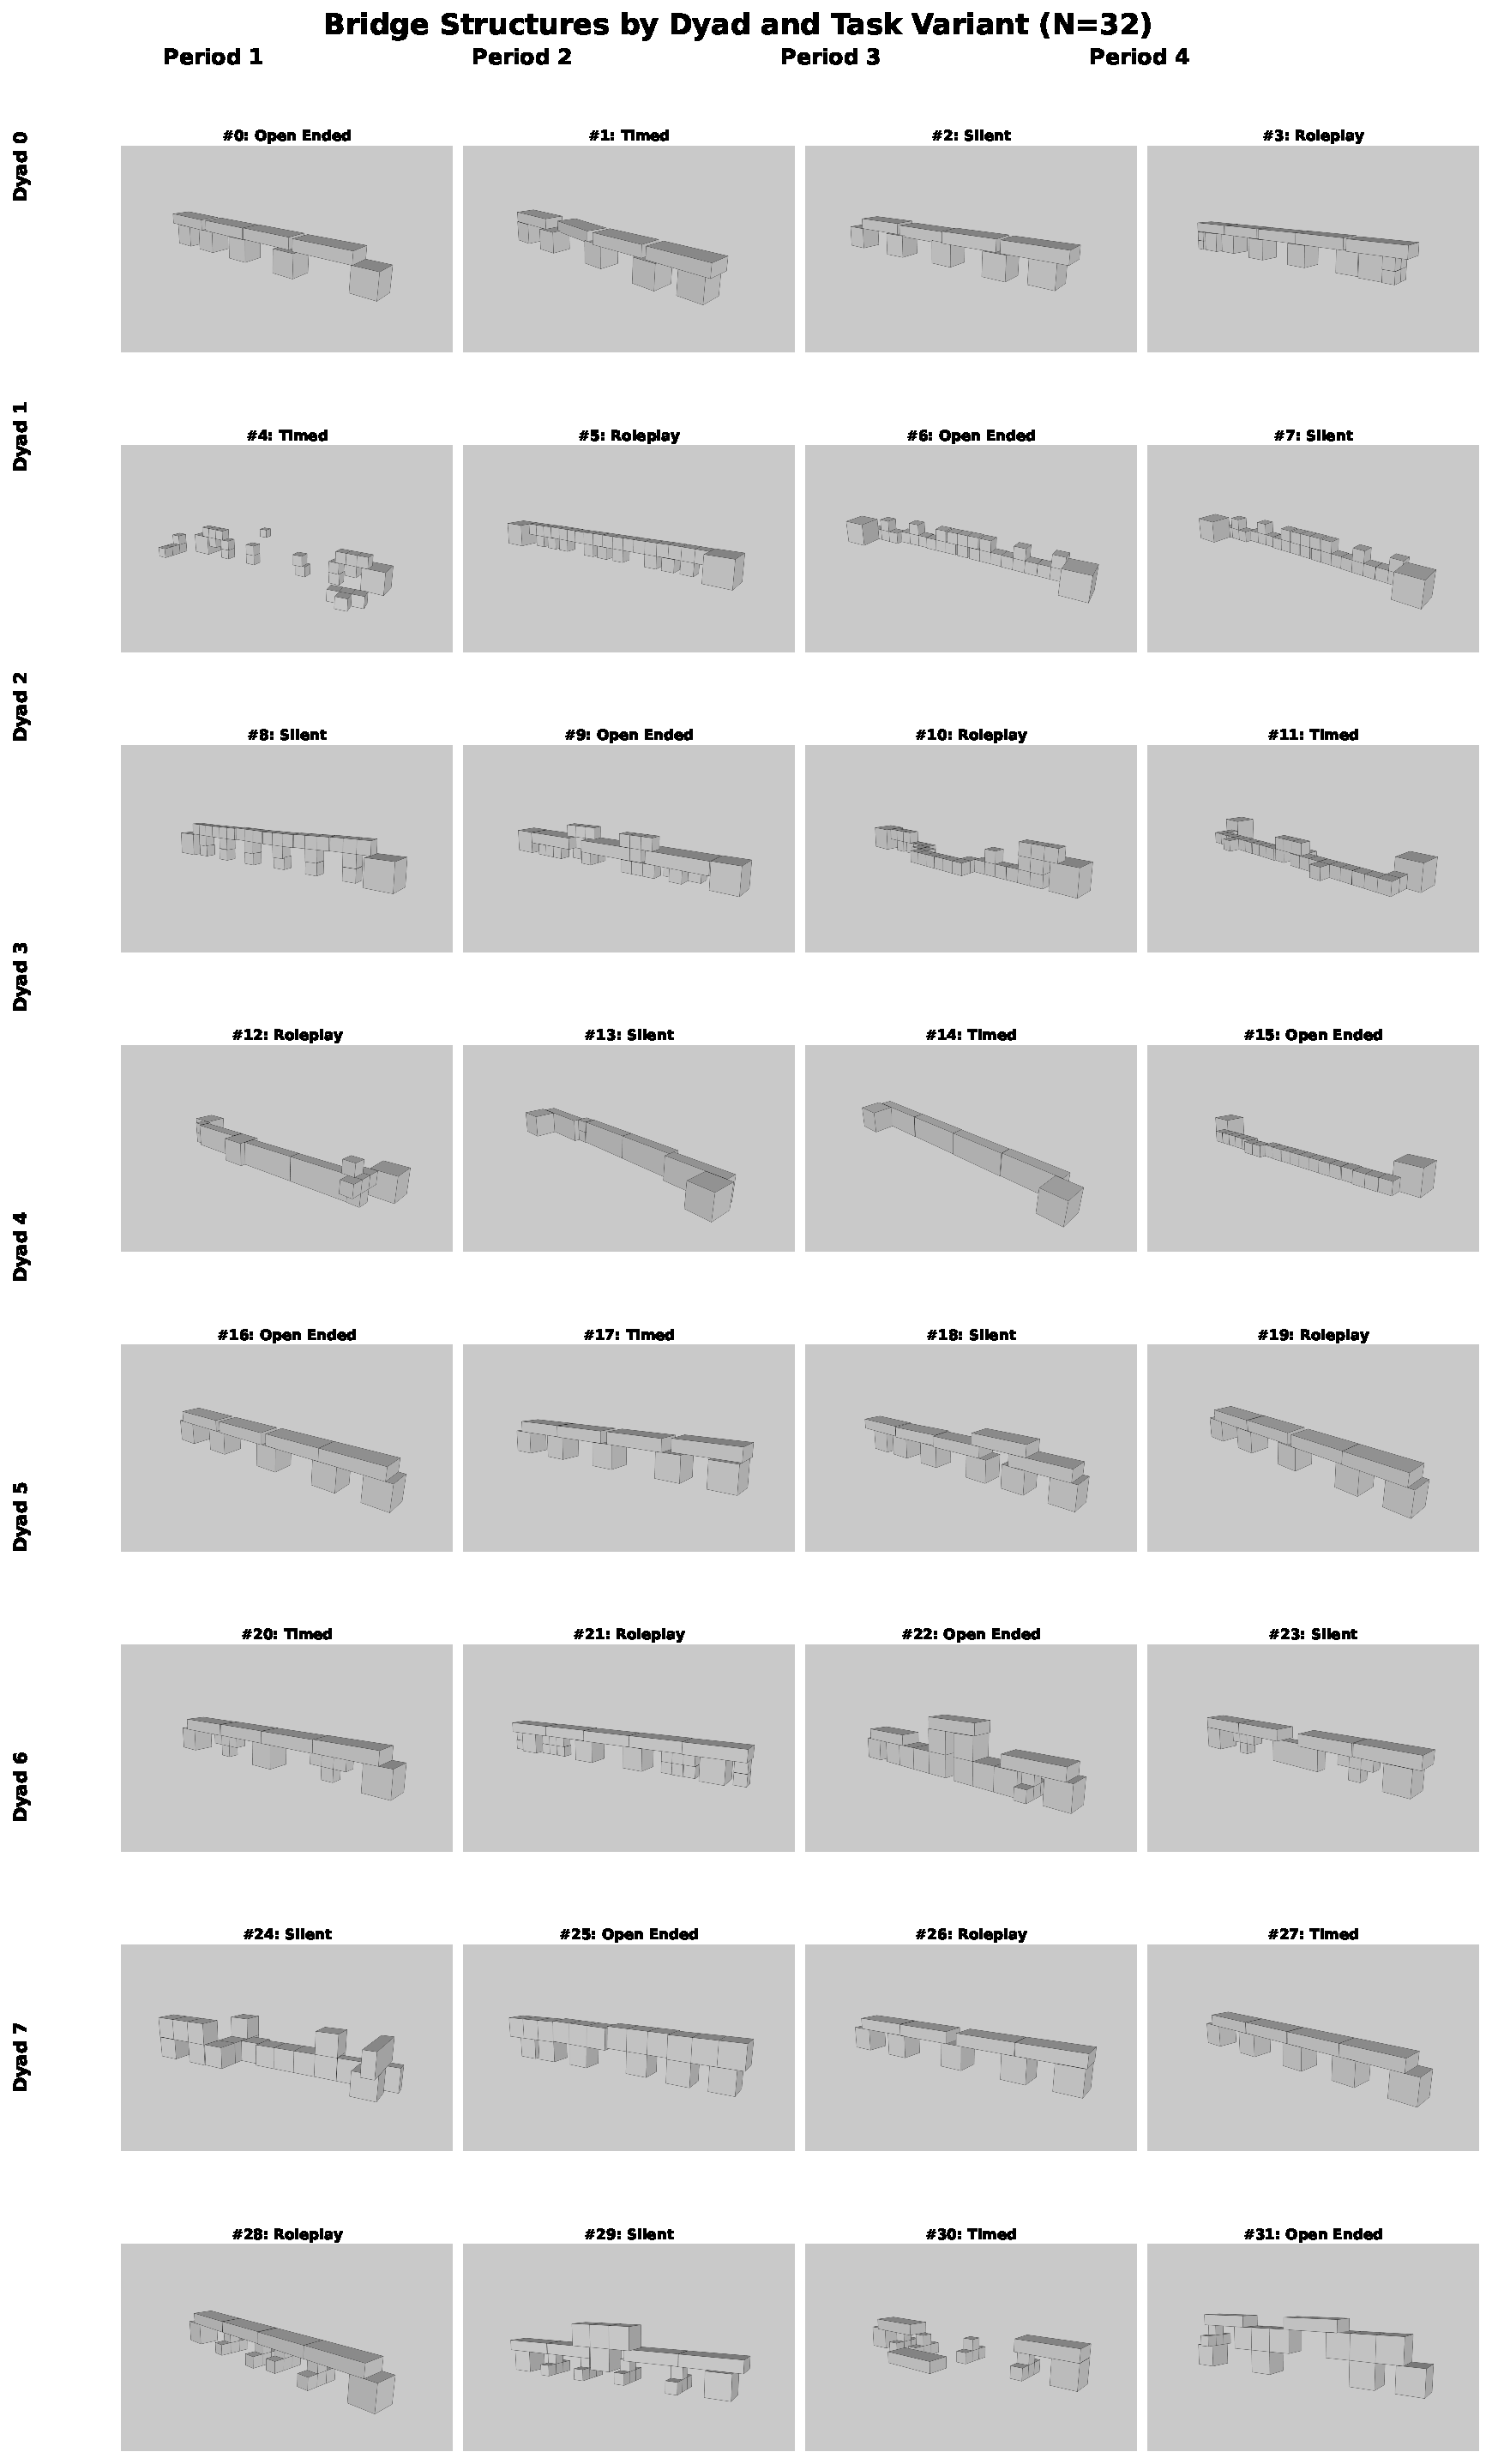
\includegraphics[width=\textwidth]{assets/06/bridge_structures_grid.pdf}
\caption{Complete overview of all 32 bridge structures organized by dyad and experimental period. Each dyad followed a different Latin square sequence, so columns represent different task variants for each row.}
\label{fig:bridge_structures_grid}
\end{figure}


\subsection{Complete Structural Analysis Data}
\begin{table}[H]
\centering
\caption{Bridge Quality Metrics - Complete Dataset (N=30 valid bridges)}
\label{tab:bridge_quality_complete}
\begin{tabular}{lrrrrrr}
\toprule
\textbf{Metric} & \textbf{N} & \textbf{Mean} & \textbf{SD} & \textbf{Median} & \textbf{Min} & \textbf{Max} \\
\midrule
Safety Factor & 30 & 10.36 & 5.01 & 13.05 & 0.49 & 15.00 \\
von Mises Stress (MPa) & 30 & 121.43 & 306.71 & 22.03 & 0.00 & 1212.00 \\
Displacement (mm) & 30 & 268,132.70 & 1,466,543.31 & 0.05 & 0.00 & 8,032,961.00 \\
Price (cost units) & 30 & 59.73 & 40.51 & 57.50 & 14.00 & 186.00 \\
Height (cm) & 30 & 30.33 & 9.28 & 30.00 & 10.00 & 50.00 \\
Total Objects & 30 & 10.17 & 3.39 & 9.00 & 6.00 & 21.00 \\
Different Object Types & 30 & 2.20 & 0.71 & 2.00 & 1.00 & 4.00 \\
\bottomrule
\end{tabular}
\end{table}

\begin{table}[H]
\centering
\caption{Bridge Quality by Collaboration Variant - Detailed Statistics}
\label{tab:bridge_quality_by_variant_complete}
\begin{tabular}{llrrrr}
\toprule
\textbf{Metric} & \textbf{Variant} & \textbf{N} & \textbf{Mean} & \textbf{SD} & \textbf{Median} \\
\midrule
\multirow{4}{*}{Safety Factor} & Open Ended & 8 & 10.95 & 5.30 & 13.56 \\
& Silent & 8 & 7.70 & 5.34 & 6.84 \\
& Timed & 6 & 10.51 & 4.92 & 10.64 \\
& Roleplay & 8 & 12.32 & 4.14 & 14.14 \\
\midrule
\multirow{4}{*}{von Mises Stress (MPa)} & Open Ended & 8 & 42.56 & 78.54 & 15.28 \\
& Silent & 8 & 229.11 & 416.64 & 37.72 \\
& Timed & 6 & 221.10 & 485.66 & 33.96 \\
& Roleplay & 8 & 17.86 & 19.00 & 15.81 \\
\midrule
\multirow{4}{*}{Displacement (mm)} & Open Ended & 8 & 1,377.02 & 3,894.66 & 0.05 \\
& Silent & 8 & 1,004,120.30 & 2,840,080.53 & 0.09 \\
& Timed & 6 & 0.28 & 0.38 & 0.15 \\
& Roleplay & 8 & 0.09 & 0.21 & 0.02 \\
\midrule
\multirow{4}{*}{Construction Cost} & Open Ended & 8 & 62.63 & 48.29 & 53.0 \\
& Silent & 8 & 71.75 & 55.21 & 67.0 \\
& Timed & 6 & 52.33 & 23.06 & 58.0 \\
& Roleplay & 8 & 50.38 & 26.79 & 54.5 \\
\bottomrule
\end{tabular}
\end{table}

\subsection{Quality-Performance Correlation Analysis}

\begin{table}[H]
\centering
\caption{Bridge Quality vs Performance Correlations}
\label{tab:quality_performance_correlations}
\begin{tabular}{lrrr}
\toprule
\textbf{Quality Metric} & \textbf{vs Completion Time} & \textbf{vs Total Objects} & \textbf{vs Efficiency} \\
\midrule
Safety Factor & r = 0.093 (p = 0.625) & r = 0.121 (p = 0.523) & r = 0.089 (p = 0.642) \\
von Mises Stress & r = -0.202 (p = 0.284) & r = -0.156 (p = 0.411) & r = -0.112 (p = 0.558) \\
Displacement & r = 0.017 (p = 0.929) & r = -0.089 (p = 0.642) & r = 0.045 (p = 0.814) \\
Construction Cost & r = 0.025 (p = 0.895) & r = 0.489 (p = 0.006**) & r = 0.156 (p = 0.411) \\
\bottomrule
\end{tabular}
\small
**p < 0.01
\end{table}

\begin{table}[H]
\centering
\caption{Statistical Tests for Bridge Quality by Variant}
\label{tab:bridge_quality_tests_complete}
\begin{tabular}{lrrrl}
\toprule
\textbf{Metric} & \textbf{$\chi^2$ (Friedman)} & \textbf{df} & \textbf{p-value} & \textbf{Kendall's W} \\
\midrule
Safety Factor & 4.062 & 3 & 0.255 & 0.226 (medium) \\
von Mises Stress & 3.200 & 3 & 0.362 & 0.178 (medium) \\
Displacement & 2.288 & 3 & 0.515 & 0.127 (medium) \\
Construction Cost & 3.120 & 3 & 0.373 & 0.173 (medium) \\
Total Objects & 2.062 & 3 & 0.560 & 0.115 (small) \\
Bridge Height & 1.875 & 3 & 0.599 & 0.104 (small) \\
\bottomrule
\end{tabular}
\end{table}

% ============================================================================
\section{Collaboration Dynamics - Detailed Results}  
\label{appendix:movement_results}
% ============================================================================

This section provides comprehensive analysis of movement patterns, spatial coordination, and collaboration dynamics across all task variants. The analysis includes partner synchronization metrics, statistical comparisons of movement efficiency, and relationships between movement patterns and task performance.

\subsection{Movement Patterns and Spatial Coordination}

This section presents the complete movement analysis including activity synchronization patterns between partners and statistical comparisons across task variants. Movement data was captured at 1Hz throughout all sessions and analyzed for coordination patterns, speed consistency, and individual differences.

\begin{table}[H]
\centering
\caption{Movement Analysis - Detailed Statistics by Variant}
\label{tab:movement_complete_stats}
\begin{tabular}{lrrrrr}
\toprule
\textbf{Variant} & \textbf{Avg Speed (m/min)} & \textbf{SD} & \textbf{Correlation (r)} & \textbf{p-value} & \textbf{Asymmetry} \\
\midrule
Open Ended & 20.75 & 8.69 & 0.890 & 0.003** & 0.22 \\
Silent & 23.02 & 8.83 & 0.351 & 0.394 & 0.24 \\
Timed & 29.38 & 12.51 & 0.939 & 0.001** & 0.18 \\
Roleplay & 22.29 & 13.68 & 0.658 & 0.076 & 0.71 \\
\midrule
\textbf{Overall} & 23.86 & 10.56 & 0.737 & < 0.001*** & 0.34 \\
\bottomrule
\end{tabular}
\small
*p < 0.05, **p < 0.01, ***p < 0.001
\end{table}

\begin{table}[H]
\centering
\caption{Individual Dyad Movement Synchronization Patterns}
\label{tab:dyad_movement_complete}
\begin{tabular}{lrrrrl}
\toprule
\textbf{Dyad} & \textbf{Correlation (r)} & \textbf{p-value} & \textbf{r²} & \textbf{Sessions} & \textbf{Coordination Level} \\
\midrule
SAKl2Kyg-jFYQhuSp & 0.996 & 0.004** & 0.992 & 4 & Near-perfect \\
kDp3Cy37-wocE408P & 0.988 & 0.012* & 0.976 & 4 & Near-perfect \\
OYYOwkG2-dckk6p6S & 0.984 & 0.016* & 0.968 & 4 & Very high \\
uTSV9lZx-iB6kR2uo & 0.945 & 0.055 & 0.893 & 4 & High \\
YeUp7E4D-WzyEiaaj & 0.753 & 0.247 & 0.567 & 4 & Moderate \\
Oa3Qww1v-zIDJJG4M & 0.718 & 0.282 & 0.516 & 4 & Moderate \\
6m7xtdFy-kHxWHBLy & 0.493 & 0.507 & 0.243 & 4 & Low \\
j7hHkgiC-iN9X5S4Q & 0.009 & 0.991 & 0.000 & 4 & Minimal \\
\bottomrule
\end{tabular}
\end{table}

\subsection{Statistical Tests for Movement Patterns}
\label{appendix:movement_communication}

This subsection provides the complete statistical test results for movement patterns, including Friedman tests for variant comparisons, correlation analyses for partner synchronization, and relationships between movement patterns and task performance.

\begin{table}[H]
\centering
\caption{Movement Pattern Statistical Analysis}
\label{tab:movement_tests_complete}
\begin{tabular}{lrrrl}
\toprule
\textbf{Analysis} & \textbf{Test Statistic} & \textbf{df} & \textbf{p-value} & \textbf{Effect/Interpretation} \\
\midrule
\textbf{Movement Efficiency by Variant} & $\chi^2 = 3.750$ & 3 & 0.290 & No significant differences \\
\textbf{Total Movement by Variant} & $\chi^2 = 7.875$ & 3 & 0.049* & Confounded by duration \\
\textbf{Partner Correlation Overall} & r = 0.737 & & < 0.001*** & Strong synchronization \\
\textbf{Movement vs Performance} & r = -0.332 & & 0.064 & Marginal negative correlation \\
\textbf{Learning Effect (Position)} & r = 0.071 & & 0.703 & No learning in movement \\
\bottomrule
\end{tabular}
\end{table}

% ============================================================================
\section{Communication Patterns - Detailed Results}
\label{appendix:communication_results}
% ============================================================================

This section presents detailed communication analysis including volume measures, turn-taking patterns, spatial language usage, and content categorization across the three verbal task variants (Open Ended, Timed, and Roleplay). The Silent condition is excluded from communication analysis by design.

\subsection{Complete Communication Analysis}

This section provides comprehensive communication analysis including word counts, turn patterns, spatial language usage, and correlations between communication measures and task performance. Analysis covers 24 sessions with verbal communication (Silent condition excluded by design).

\begin{table}[H]
\centering
\caption{Communication Patterns - Complete Statistics by Variant}
\label{tab:communication_complete_stats}
\begin{tabular}{lrrrrr}
\toprule
\textbf{Metric} & \textbf{Open Ended} & \textbf{Timed} & \textbf{Roleplay} & \textbf{Test Stat} & \textbf{p-value} \\
\midrule
Total Words (mean ± SD) & 472 ± 303 & 341 ± 303 & 1172 ± 1142 & $\chi^2 = 9.750$ & 0.008** \\
Words per Minute & 65.1 ± 30.9 & 69.8 ± 31.1 & 77.7 ± 36.1 & $\chi^2 = 0.750$ & 0.687 \\
Turns per Minute & 10.7 ± 4.1 & 9.8 ± 2.8 & 9.9 ± 3.3 & $\chi^2 = 2.250$ & 0.325 \\
Communication Balance & 0.39 ± 0.25 & 0.51 ± 0.36 & 0.33 ± 0.30 & $\chi^2 = 1.750$ & 0.417 \\
Deictic Density (\%) & 6.8 ± 1.4 & 6.1 ± 2.0 & 6.5 ± 1.8 & $\chi^2 = 0.250$ & 0.882 \\
Spatial Density (\%) & 2.0 ± 0.8 & 2.0 ± 0.9 & 2.0 ± 0.4 & $\chi^2 = 2.250$ & 0.325 \\
Planning Ratio (\%) & 31.7 ± 12.1 & 32.6 ± 8.2 & 32.1 ± 11.0 & $\chi^2 = 0.750$ & 0.687 \\
Turn Transitions & 22.1 ± 14.2 & 10.9 ± 9.5 & 40.6 ± 38.3 & $\chi^2 = 8.968$ & 0.011* \\
\bottomrule
\end{tabular}
\small
*p < 0.05, **p < 0.01
\end{table}

\begin{table}[H]
\centering
\caption{Communication Volume and Performance Relationships}
\label{tab:communication_performance_complete}
\begin{tabular}{lrrr}
\toprule
\textbf{Relationship} & \textbf{Correlation (r)} & \textbf{p-value} & \textbf{Interpretation} \\
\midrule
Total Words vs Completion Time & 0.523 & 0.009** & Positive (expected) \\
Words per Minute vs Completion Time & 0.034 & 0.873 & No relationship \\
Communication Balance vs Performance & -0.187 & 0.383 & Weak negative \\
Deictic Density vs Task Efficiency & 0.156 & 0.467 & Weak positive \\
Planning Ratio vs Bridge Quality & 0.089 & 0.678 & No relationship \\
\bottomrule
\end{tabular}
\end{table}

% ============================================================================
\section{System Performance and Subjective Experience}
\label{appendix:results:subjective}
% ============================================================================

\subsection{System Usability and Workload Progression}
\label{appendix:subjective}

\begin{table}[H]
\centering
\caption{System Usability Scale (SUS) and NASA-TLX by Session}
\label{tab:sus_tlx_complete}
\begin{tabular}{lrrrrrrr}
\toprule
\textbf{Session} & \textbf{SUS Mean} & \textbf{SUS SD} & \textbf{SUS SE} & \textbf{TLX Mean} & \textbf{TLX SD} & \textbf{TLX SE} & \textbf{N} \\
\midrule
1 & 67.5 & 11.1 & 2.8 & 7.3 & 10.8 & 2.7 & 16 \\
2 & 70.6 & 14.0 & 3.5 & 18.0 & 18.2 & 4.5 & 16 \\
3 & 69.8 & 15.4 & 3.8 & 18.0 & 23.8 & 6.0 & 16 \\
4 & 72.5 & 13.8 & 3.5 & 9.7 & 13.7 & 3.4 & 16 \\
\midrule
\textbf{Change (1→4)} & \textbf{+5.0*} & & & \textbf{+2.5} & & & \\
\textbf{Effect Size} & \textbf{d = 0.98} & & & \textbf{d = 0.19} & & & \\
\bottomrule
\end{tabular}
\small
*p < 0.05 (t = 2.760, p = 0.015)
\end{table}

\begin{table}[H]
\centering
\caption{Learning Effects by AR/VR Experience Level}
\label{tab:experience_learning_complete}
\begin{tabular}{lrrrrrr}
\toprule
\textbf{Experience} & \textbf{N} & \textbf{Initial SUS} & \textbf{Final SUS} & \textbf{Change} & \textbf{Completion Time} & \textbf{Performance} \\
\midrule
None & 3 & 67.5 ± 8.8 & 72.5 ± 6.6 & +5.0 & 7.28 ± 3.12 & Baseline \\
Limited & 6 & 64.2 ± 11.8 & 73.8 ± 15.6 & +9.6 & 7.85 ± 2.89 & Similar \\
Moderate & 5 & 72.5 ± 10.4 & 71.5 ± 15.1 & -1.0 & 8.48 ± 3.21 & Slowest \\
Extensive & 2 & 81.3 ± 12.4 & 87.5 ± 3.5 & +6.2 & 6.41 ± 2.15 & Fastest \\
\bottomrule
\end{tabular}
\end{table}

\subsection{Relationship and Trust Measures}

\begin{table}[H]
\centering
\caption{Interpersonal Relationship Measures Pre-Post Study}
\label{tab:relationship_measures_complete}
\begin{tabular}{lrrrrl}
\toprule
\textbf{Measure} & \textbf{Pre-Study} & \textbf{Post-Study} & \textbf{Change} & \textbf{p-value} & \textbf{Effect} \\
\midrule
IOS (Inclusion of Other in Self) & 3.69 ± 1.25 & 3.75 ± 1.18 & +0.06 & 0.789 & No change \\
Partner Competence Rating & 4.2 ± 0.8 & 4.3 ± 0.7 & +0.1 & 0.678 & No change \\
Collaboration Satisfaction & N/A & 4.1 ± 0.9 & N/A & N/A & High satisfaction \\
\bottomrule
\end{tabular}
\end{table}

% ============================================================================
\section{Individual Differences and Personality Effects}
\label{appendix:individual_differences}
% ============================================================================

\begin{table}[H]
\centering
\caption{Personality-Performance Correlation Matrix}
\label{tab:personality_complete}
\begin{tabular}{lrrrrr}
\toprule
\textbf{Big Five Trait} & \textbf{Completion Time} & \textbf{Bridge Quality} & \textbf{SUS Score} & \textbf{Movement Sync} & \textbf{Communication} \\
\midrule
Openness & -0.409 (0.115) & 0.122 (0.657) & 0.234 (0.386) & 0.067 (0.805) & 0.156 (0.572) \\
Conscientiousness & -0.009 (0.974) & 0.089 (0.741) & 0.156 (0.563) & -0.234 (0.386) & -0.089 (0.741) \\
Extraversion & -0.111 (0.682) & -0.034 (0.900) & 0.301 (0.256) & 0.178 (0.512) & 0.234 (0.386) \\
Agreeableness & -0.036 (0.895) & 0.201 (0.456) & 0.189 (0.483) & 0.089 (0.741) & -0.067 (0.805) \\
Neuroticism & -0.116 (0.668) & -0.156 (0.563) & -0.223 (0.408) & -0.112 (0.682) & 0.023 (0.932) \\
\bottomrule
\end{tabular}
\small
Values shown as r (p-value). No correlations reach statistical significance.
\end{table}

\begin{table}[H]
\centering
\caption{Demographic Effects on Performance}
\label{tab:demographics_performance_complete}
\begin{tabular}{lrrrrr}
\toprule
\textbf{Factor} & \textbf{N} & \textbf{Completion Time} & \textbf{Bridge Quality} & \textbf{SUS Progression} & \textbf{Notes} \\
\midrule
\textbf{Gender} & & & & & \\
Male & 10 & 7.59 ± 2.83 & 10.2 ± 4.8 & +4.8 & Similar performance \\
Female & 6 & 7.89 ± 3.50 & 10.6 ± 5.4 & +5.3 & Similar performance \\
\midrule
\textbf{Age Correlation} & 16 & r = 0.424 (0.101) & r = -0.156 (0.563) & r = -0.089 (0.741) & Marginal age effect \\
\midrule
\textbf{Language} & & & & & \\
German & 13 & 7.68 ± 2.94 & 10.5 ± 4.9 & +5.2 & Majority group \\
Other & 3 & 7.93 ± 4.11 & 9.8 ± 5.8 & +4.0 & Small sample \\
\bottomrule
\end{tabular}
\end{table}

% ============================================================================
\section{Construction Efficiency and Material Usage}
\label{appendix:construction}
% ============================================================================

\begin{table}[H]
\centering
\caption{Construction Efficiency and Resource Usage by Variant}
\label{tab:construction_complete}
\begin{tabular}{lrrrrrr}
\toprule
\textbf{Variant} & \textbf{Objects Used} & \textbf{Objects Spawned} & \textbf{Efficiency} & \textbf{Waste \%} & \textbf{Types Used} & \textbf{N} \\
\midrule
Open Ended & 10.1 ± 3.2 & 22.2 ± 8.1 & 0.478 ± 0.113 & 52.2 & 2.38 ± 0.74 & 8 \\
Silent & 10.0 ± 2.8 & 19.0 ± 7.2 & 0.638 ± 0.323 & 36.2 & 2.00 ± 0.53 & 8 \\
Timed & 8.5 ± 2.1 & 11.7 ± 4.3 & 0.810 ± 0.335 & 19.0 & 2.00 ± 0.63 & 6 \\
Roleplay & 11.6 ± 4.1 & 26.2 ± 9.8 & 0.524 ± 0.259 & 47.6 & 2.71 ± 0.95 & 8 \\
\bottomrule
\end{tabular}
\end{table}

\begin{table}[H]
\centering
\caption{Building Block Type Preferences by Variant (\% of spawned objects)}
\label{tab:block_preferences_complete}
\begin{tabular}{lrrrr}
\toprule
\textbf{Block Type} & \textbf{Open Ended} & \textbf{Silent} & \textbf{Timed} & \textbf{Roleplay} \\
\midrule
BigTShape & 12.4 & 4.6 & 1.4 & 1.0 \\
Cube & 9.6 & 11.8 & 24.3 & 21.0 \\
Plank & 19.1 & 35.5 & 48.6 & 28.1 \\
SmallCube & 27.5 & 13.8 & 1.4 & 27.6 \\
BigLShape & 6.7 & 2.0 & 1.4 & 0.0 \\
TShape & 20.2 & 32.2 & 2.9 & 17.1 \\
LShape & 4.5 & 0.0 & 20.0 & 5.2 \\
\bottomrule
\end{tabular}
\end{table}

% ============================================================================
\section{Statistical Power Analysis and Effect Sizes}
\label{appendix:power_analysis}
% ============================================================================

\begin{table}[H]
\centering
\caption{Power Analysis Results for Key Statistical Tests}
\label{tab:power_analysis_complete}
\begin{tabular}{lrrrl}
\toprule
\textbf{Test Type} & \textbf{Sample Size} & \textbf{Observed Power} & \textbf{Effect Size} & \textbf{Interpretation} \\
\midrule
\textbf{Friedman Test (n=8 dyads, 4 conditions)} & & & & \\
Small effects (f = 0.25) & 8 & 0.14 & Kendall's W = 0.14 & Underpowered \\
Medium effects (f = 0.40) & 8 & 0.34 & Kendall's W = 0.34 & Underpowered \\
Large effects (f = 0.60) & 8 & 0.71 & Kendall's W = 0.53 & Adequate for large effects \\
\midrule
\textbf{Wilcoxon Signed-Rank (n=8 pairs)} & & & & \\
Medium effects (d = 0.5) & 8 & 0.19 & r = 0.46 & Underpowered \\
Large effects (d = 0.8) & 8 & 0.43 & r = 0.80 & Marginal power \\
Very large effects (d = 1.3) & 8 & 0.80 & r = 0.94 & Adequate power \\
\midrule
\textbf{Correlation Analysis (n=16 individuals)} & & & & \\
Medium correlations (r = 0.5) & 16 & 0.51 & & Underpowered \\
Large correlations (r = 0.7) & 16 & 0.88 & & Adequate power \\
\bottomrule
\end{tabular}
\end{table}

% ============================================================================
% \section{Key Statistical Results Summary}
% \label{appendix:stats_summary}
% % ============================================================================

% \subsection{Significant Effects (p < 0.05)}
% \begin{itemize}
% \item \textbf{Collaboration variant on completion time}: Friedman $\chi^2$ = 12.750, p = 0.005, Kendall's W = 0.531 (large effect)
% \item \textbf{Silent vs verbal communication}: Mann-Whitney U = 27.0, p = 0.025, r = 0.46 (medium effect)
% \item \textbf{Roleplay vs other variants}: Multiple comparisons p < 0.05, large effect sizes (r > 0.8)
% \item \textbf{Total communication volume by variant}: Friedman $\chi^2$ = 9.750, p = 0.008
% \item \textbf{Turn transitions by variant}: Friedman $\chi^2$ = 8.968, p = 0.011
% \item \textbf{Movement synchronization overall}: r = 0.737, p < 0.001 (large effect)
% \item \textbf{SUS learning effect}: t = 2.760, p = 0.015, Cohen's d = 0.98 (large effect)
% \end{itemize}

% \subsection{Non-significant Effects (p > 0.05)}
% \begin{itemize}
% \item Virtual environment on any performance metric (p = 0.522)
% \item Task position (learning) on completion time overall (p = 0.440)
% \item Bridge quality metrics by collaboration variant (all p > 0.25)
% \item Personality traits on task performance (all p > 0.10)
% \item NASA-TLX workload changes across sessions (p = 0.597)
% \item Movement efficiency by variant (p = 0.290)
% \item Communication density and spatial reference patterns by variant
% \end{itemize}

% \subsection{Effect Sizes and Practical Significance}
% \begin{itemize}
% \item \textbf{Communication paradox}: Silent condition 2.2× faster than verbal conditions
% \item \textbf{Time pressure effect}: Timed variant 3.1× faster than untimed variants
% \item \textbf{Role conflict overhead}: Roleplay variant 2.6× slower with 2.2× more movement
% \item \textbf{Movement synchronization}: Strongest effect in study (r = 0.737, large effect)
% \item \textbf{Quality-speed independence}: No meaningful correlations across all quality measures
% \item \textbf{Learning effect}: 5-point SUS improvement with large effect size (d = 0.98)
% \end{itemize}

% \subsection{Interpretive Notes}
% Given the study's power limitations, non-significant findings with small-to-medium effect sizes should be considered \textbf{inconclusive} rather than evidence of no effect. The significant effects observed represent genuinely substantial differences that exceeded the study's detection threshold. All effect size interpretations follow Cohen's conventions: small (0.2), medium (0.5), large (0.8) for d; small (0.1), medium (0.3), large (0.5) for r.

\section{Communication Coding Categories}\label{appendix:coding_categories}

This section documents the specific word lists and coding schemes used for transcript analysis presented in Section~\ref{sec:communication}. All word matching was performed using case-insensitive regular expressions on participant utterances (statements by host excluded).

\subsection{Spatial Reference Coding}

Spatial references were identified using two main categories: deictic references and directional/positional language.

\subsubsection{Deictic Reference Patterns}
Basic spatial deixis patterns using regular expressions:
\begin{itemize}
\item \texttt{\\b(here|there|this|that)\\b} - Basic spatial demonstratives
\item \texttt{\\b(left|right|up|down|over|under)\\b} - Directional terms
\item \texttt{\\b(next to|beside|behind|in front)\\b} - Relational positioning
\item \texttt{\\b(put|place|move|go)\\s+(it|this|that|there|here)\\b} - Action-location combinations
\item \texttt{\\b(on|in|at|to|from)\\s+(the|this|that)\\b} - Prepositional references
\end{itemize}

\subsubsection{Calculation Method}
Spatial reference density was calculated as:
$$\text{Spatial Density} = \frac{\text{Total Spatial References}}{\text{Total Words in Session}}$$

This metric represents the proportion of words dedicated to spatial coordination language.

\subsection{Planning vs. Execution Communication}

Communication was categorized into planning-oriented and execution-oriented language based on distinct word patterns.

\subsubsection{Planning Language Patterns}
Planning-related communication included three subcategories:

\textbf{Strategy and Deliberation:}
\begin{itemize}
\item \texttt{plan}, \texttt{strategy}, \texttt{should}, \texttt{let's}, \texttt{how about}, \texttt{what if}, \texttt{we could}
\end{itemize}

\textbf{Temporal Sequencing:}
\begin{itemize}
\item \texttt{first}, \texttt{then}, \texttt{next}, \texttt{after}, \texttt{before}
\end{itemize}

\textbf{Ideation and Reflection:}
\begin{itemize}
\item \texttt{idea}, \texttt{think}, \texttt{suggest}, \texttt{propose}
\end{itemize}

\subsubsection{Execution Language Patterns}
Execution-related communication included three subcategories:

\textbf{Direct Actions:}
\begin{itemize}
\item \texttt{put}, \texttt{place}, \texttt{move}, \texttt{grab}, \texttt{take}, \texttt{drop}
\end{itemize}

\textbf{Immediate Coordination:}
\begin{itemize}
\item \texttt{there}, \texttt{here}, \texttt{now}, \texttt{wait}, \texttt{good}, \texttt{done}
\end{itemize}

\textbf{Confirmation and Response:}
\begin{itemize}
\item \texttt{yes}, \texttt{no}, \texttt{ok}, \texttt{okay}, \texttt{right}, \texttt{wrong}
\end{itemize}

\subsubsection{Calculation Method}
Planning ratio was calculated as:
$$\text{Planning Ratio} = \frac{\text{Planning Utterances}}{\text{Planning Utterances + Execution Utterances}}$$

Only utterances containing planning or execution markers were included in this ratio calculation.

\subsection{Content Theme Analysis}

Additional thematic content analysis used the following categories:

\textbf{Building Actions:}
\begin{itemize}
\item \texttt{build}, \texttt{place}, \texttt{put}, \texttt{move}, \texttt{position}, \texttt{block}, \texttt{cube}, \texttt{plank}
\end{itemize}

\textbf{Planning and Strategy:}
\begin{itemize}
\item \texttt{plan}, \texttt{strategy}, \texttt{idea}, \texttt{think}, \texttt{should}, \texttt{could}, \texttt{would}, \texttt{maybe}
\end{itemize}

\textbf{Spatial Coordination:}
\begin{itemize}
\item \texttt{here}, \texttt{there}, \texttt{this}, \texttt{that}, \texttt{left}, \texttt{right}, \texttt{side}, \texttt{middle}
\end{itemize}

\textbf{Evaluation and Quality:}
\begin{itemize}
\item \texttt{good}, \texttt{bad}, \texttt{better}, \texttt{worse}, \texttt{price}, \texttt{cost}, \texttt{strong}, \texttt{stable}
\end{itemize}

\textbf{Problem Identification:}
\begin{itemize}
\item \texttt{problem}, \texttt{issue}, \texttt{wrong}, \texttt{error}, \texttt{stuck}, \texttt{difficult}, \texttt{help}
\end{itemize}

\textbf{Agreement and Acknowledgment:}
\begin{itemize}
\item \texttt{yes}, \texttt{okay}, \texttt{right}, \texttt{sure}, \texttt{agree}, \texttt{no}, \texttt{wait}
\end{itemize}

\subsection{Implementation Details}

All coding was implemented using Python regular expressions with the following considerations:
\begin{itemize}
\item Word boundary matching (\texttt{\\b}) to avoid partial word matches
\item Case-insensitive matching for consistent results
\item Substring matching for morphological variations (e.g., "building" matches "build")
\item Exclusion of HOST utterances from all participant communication metrics
\end{itemize}

The analysis scripts are available in the \texttt{user-study-analysis/} directory, with primary implementations in \texttt{transcript\_analysis.py} and \texttt{communication\_analysis.py}.

